% ----- Start of translated content from: part_01.tex -----

\documentclass[11pt, a4paper, oneside]{article}

% --- 必要的宏包 ---
\usepackage{graphicx} % 用于插入图像(徽标)
% 调整页边距以为页眉留出更多空间
\usepackage[a4paper, top=4cm, bottom=2.5cm, left=2.5cm, right=2.5cm, headheight=1.2cm, headsep=1.5cm]{geometry}
\usepackage{xcolor} % 定义并使用自定义颜色
\usepackage{titlesec} % 自定义章节标题
\usepackage{enumitem} % 自定义列表
\usepackage{hyperref} % 创建内部与外部链接
\usepackage{ragged2e} % 改善文本对齐
\usepackage{lettrine} % 首字下沉
\usepackage{fancyhdr} % 自定义页眉与页脚
\usepackage{tabularx} % 固定宽度的表格
\usepackage{amsfonts} % 数学符号(如需)
\usepackage{amsmath}
\usepackage[utf8]{inputenc}
\usepackage{graphicx}
\usepackage{booktabs}
\usepackage{tikz}
\usepackage{pgfplots}
\usepackage{float}
\usepackage{eurosym}
\usepackage{microtype}
\usepackage{siunitx} 
\pgfplotsset{compat=1.18}
% --- 字体与语言设置(需要 XeLaTeX) ---
\usepackage{fontspec}
\usepackage{xeCJK}
\usepackage{multirow}
\usepackage{booktabs,longtable,siunitx,ragged2e,placeins} 

\def\UrlBreaks{\do\.\do\/\do\-\do\_\do\?\do\&} % 允许在 URL 中断行
\newcolumntype{L}{>{\raggedright\arraybackslash}X} % 变宽列,文本左对齐


% 直接从本地文件加载字体,并指定不同字重。
% 这是最稳健的方法。
% 确保 .ttf 文件位于名为“fonts”的子文件夹中。
\setmainfont{NotoSans-Regular.ttf}[
    Path = ./fonts/,
    BoldFont = NotoSans-Bold.ttf,
    ItalicFont = NotoSans-Italic.ttf,
    BoldItalicFont = NotoSans-BoldItalic.ttf
]
\setCJKmainfont{NotoSansSC-Regular.ttf}[
    Path = ./fonts/,
    BoldFont = NotoSansSC-Bold.ttf,
    ItalicFont = NotoSansSC-Regular.ttf
]
% 定义一个新的“light”字体以供自定义使用
\newfontfamily\lightfont{NotoSans-Light.ttf}[
    Path = ./fonts/,
    ItalicFont = NotoSans-LightItalic.ttf
]



% --- 品牌颜色定义(可自定义) ---
\definecolor{PrimaryColor}{HTML}{6A4C9C}   % 主色(如紫色)
\definecolor{SecondaryColor}{HTML}{2A2F45} % 次要颜色(如深蓝)
\definecolor{AccentColor}{HTML}{8E7CC3}    % 强调色
\definecolor{DarkGray}{HTML}{343a40}      % 文本深灰

% --- hyperref 设置 ---
\hypersetup{
    colorlinks=true,
    linkcolor=PrimaryColor,
    filecolor=AccentColor,      
    urlcolor=SecondaryColor,
    citecolor=AccentColor,
    pdftitle={商业计划书},
    pdfpagemode=FullScreen,
}

% --- 章节标题个性化 ---
\titleformat{\section}
  {\normalfont\Large\bfseries\color{SecondaryColor}}
  {\thesection}{1em}{}
\titleformat{\subsection}
  {\normalfont\large\bfseries\color{PrimaryColor}}
  {\thesubsection}{1em}{}
\titleformat{\subsubsection}
  {\normalfont\normalsize\bfseries\color{AccentColor}}
  {\thesubsubsection}{1em}{}

% --- 头部和页脚设置 ---
\pagestyle{fancy}
\fancyhf{} % 清空所有页眉和页脚字段
% 将页眉的文本置于左侧,徽标置于右侧
\fancyhead[L]{\textcolor{PrimaryColor}{\small 商业计划书}}
\fancyhead[R]{
\includegraphics[height=0.8cm]{IntellyHub_Logo_Colored.png}}
\fancyfoot[C]{\textcolor{DarkGray}{\thepage}}
\renewcommand{\headrulewidth}{0.4pt}
\renewcommand{\footrulewidth}{0.4pt}
\renewcommand{\headrule}{\color{PrimaryColor}\hrule}
\renewcommand{\footrule}{\color{PrimaryColor}\hrule}


% --- 文档开始 ---
\begin{document}
% --- 标题页 ---
% 第一页使用 'empty' 样式以不显示页眉
\thispagestyle{empty} 
\begin{titlepage}
    \centering
    \vspace{1cm}
    
    % 插入徽标(将 'logo.png' 替换为你的文件)
    
\includegraphics[width=0.6\textwidth]{IntellyHub_Logo_Colored.png}
    
    \vspace{2.5cm}
    
    % 文档标题
    {\Huge\bfseries\color{PrimaryColor}商业计划书}
    
    \vspace{1.5cm}
    
    % 副标题使用轻体的示例
    {\Large\itshape\lightfont 会思考的自动化。}
    
    \vfill % 可伸缩的垂直间距
    
    % 公司信息和日期
    {\large\bfseries\color{PrimaryColor}v2.02 \color{SecondaryColor}商业计划书}
    
    \vspace{0.5cm}
    
    {\large \today}
    
\end{titlepage}

% --- 目录 ---
\tableofcontents
\newpage

% --- 商业计划书的各部分 ---

\section{执行摘要}
IntellyHub 是一个 AI 工作流与代理编排平台,使组织能够构建、部署并管理复杂的 AI 驱动工作流和自主代理。它通过提供一个统一的 \textbf{企业级平台} 来编排多种 AI 模型(LLMs)、MCP 服务器、检索-增\-强\-生成(RAG)流水线、自定义 Python 逻辑以及传统应用集成,弥合了传统自动化工具与前沿 AI 框架之间的鸿沟。 

该平台的可视化/代码混合式 IDE 和可扩展插件体系,使 AI 工程师与 DevOps 团队无需深厚的基础设施专业知识即可将 AI 解决方案运营化。 

IntellyHub 的 \textbf{以产品驱动的增长战略}(免费层和自助工具)旨在推动开发者的快速采用,并在使用规模扩大时转化为付费方案。鉴于 AI 自动化/AutoML 与 MLOps 市场的爆炸式增长(48,3\% 年增长率\cite{AIMarket} 和 39,8\%\cite{MLOpsMarket}),IntellyHub 通过提供企业所需的 \textbf{安全性、治理与可扩展性},同时满足开发者所需的灵活性,有望抓住这一融合趋势。

我们预计未来三年将实现强劲的用户采用与收入增长,这一趋势由面向 AI/ML 工程用例的高价值 SaaS 商业模式所支撑。

\section{公司介绍}
\subsection{使命宣言}
IntellyHub 的使命是通过提供一个统一的平台来编排复杂工作流与自主代理,帮助组织充分释放 AI 的潜能。我们的目标是弥合传统自动化工具与前沿 AI 框架之间的差距,实现对 AI 驱动解决方案的无缝集成与管理。

\subsection{愿景}
IntellyHub 展望一个 AI 无缝融入企业运营各个方面的未来,使组织能够自动化复杂任务、强化决策并推动创新。我们致力于成为 AI 工作流编排的领先平台,赋能开发者与企业构建能够变革行业与科学研究的智能系统。

\subsection{价值观}
\begin{itemize}
    \item \textbf{创新:} 我们致力于持续创新,拓展 AI 与自动化的可能边界。
    \item \textbf{协作:} 我们相信协作的力量,无论在团队内部还是与用户协作,推动成功并创造价值。
    \item \textbf{诚信:} 我们在所有互动中恪守最高标准,确保与客户和合作伙伴之间的信任与透明。
    \item \textbf{以客户为中心:} 用户是我们一切工作的核心。我们倾听他们的需求,并努力超越其期望。

% ----- End of translated content from: part_02.tex -----

% ----- Start of translated content from: part_03.tex -----

\end{itemize}


\section{产品概览}
IntellyHub 的核心价值在于以对开发者友好且面向企业的方式,实现\textbf{高级 AI 编排}。
\begin{itemize}
    \item \textbf{混合编排 IDE:} 基于 Web 的界面提供两种同步视图——\textbf{基于可视化节点的“Design”视图与以代码为中心的“YAML/Python”视图}——用于定义工作流与智能体逻辑。该混合 IDE 支持在零代码的工作流设计与全代码自定义之间无缝切换,兼顾非技术用户与程序员。
    
    \item \textbf{可扩展 AI 插件系统:} IntellyHub 具有模块化与可扩展性。开发者可以为新的触发器(事件监听器)、动作(工作流步骤)或集成创建自定义插件。平台尤其支持用于集成各类 AI 模型(如 OpenAI、Anthropic Claude 等)、向量数据库和外部工具的插件。该插件架构使平台具备面向未来的能力,能够快速支持新兴的 AI 模型与服务。
    
    \item \textbf{用于工作流生成的 AI 智能体:} IntellyHub 内置 AI 智能体,可从自然语言自动生成工作流。为确保其知识始终最新,智能体会动态查询专用的\textbf{MCP(模型上下文协议)服务器}以获取最新可用插件及其使用说明。结合微调模型,此过程使智能体能够生成准确、可执行的工作流,充分利用平台的最新能力。
    
    \item \textbf{云原生执行引擎:} 每个自动化或智能体都运行在独立的 Kubernetes Pod 中。此设计在安全性(工作流级进程隔离)、可扩展性(Pod 可按需启动/停止)和资源治理方面具有优势——包括为 AI 密集型工作流分配 GPU 或额外内存。云原生的容器化执行确保即便是复杂的基于 LLM 的智能体也能在负载下可靠扩展,并为每次运行提供集中式监控与日志记录。
    
    \item \textbf{自动化\&智能体市场:} IntellyHub 内置预构建自动化与 AI 智能体的商店。用户可一键部署模板,或将自己的创作分享给社区。该市场促进社区驱动的生态,帮助新用户快速上手成熟模板,并为高级用户分发智能体提供渠道(提升平台粘性)。模板覆盖传统任务(如 CRM 数据同步)与高级 AI 智能体(如基于 LLM 的研究助理)。
    
    \item \textbf{团队协作功能:} IntellyHub 支持多用户团队的基于角色的访问控制、版本管理与基于 DevOps 与 MLOps 的变更跟踪。团队可高效协作构建工作流、共享模板并有效管理权限。平台还为每个工作流内置评论与讨论线程,实现实时协作与反馈。
\end{itemize}

\pagebreak
\subsection{技术栈}
IntellyHub 基于现代、稳健且可扩展的技术栈构建,以确保企业级性能、安全与开发者生产力。

\begin{itemize}
\item \textbf{前端(IDE):} 我们的核心用户体验来自高度交互的 Web 应用,使用 \textbf{Vue 3} 与 \textbf{TypeScript} 构建,并由 Vite 提供快速开发工作流。界面采用 \textbf{Vuetify} 组件库实现简洁一致的设计,使用 \textbf{Vue Flow} 构建可视化节点编辑器,并通过 \textbf{Monaco Editor} 提供专业级编码体验。

\item \textbf{后端(API \& 控制平面):} 包括主 API 与 MCP(Master Control Point)服务器在内的后端服务使用 \textbf{Python} 与轻量且强大的 \textbf{Flask} Web 框架开发。该选择便于快速迭代并与 Python 生态中的 AI 与自动化工具轻松集成。

\item \textbf{自动化\&AI 引擎:} 用于编排自动化与 AI 智能体的核心逻辑由 \textbf{Python} 实现,并基于业界标准的 \textbf{LangChain} 框架。这为创建复杂的多步 AI 工作流、管理与各类 LLM 的交互,以及确保智能体开发的模块化提供了稳固基础。

\item \textbf{基础设施与执行环境:} 整个平台运行在 \textbf{Kubernetes(K8s)} 上,作为我们的核心基础设施。每个自动化都在专用、隔离的 Pod 中执行,提供最大化的安全性与可扩展性。该云原生方法是我们面向企业价值主张的基石。
\end{itemize}

\subsection{独特价值主张}
IntellyHub 的独特价值并非来自单一功能,而是源于核心技术的协同整合,从而带来可衡量的业务成果。我们将自动化从高风险、碎片化的尝试,转变为受治理、影响深远且可量化的业务资产。

\begin{itemize}
    \item \textbf{显著降低运营风险并加速上市时间。} 我们解决了“能力”与“治理”之间的权衡。
    \begin{itemize}
        \item \textit{赋能技术:} 我们的\textbf{Kubernetes 原生执行引擎}开箱即用地提供安全、可审计、可扩展的基础。每个工作流都在专用、隔离的 Pod 中运行。
        \item \textit{可衡量影响:} 与自定义脚本相比,客户可量化地降低基础设施管理开销,缩短复杂工作流的执行时间,并将与进程隔离相关的安全漏洞降至接近零。
    \end{itemize}

    \item \textbf{打破孤岛,释放团队生产力。} 我们解决业务与技术团队之间沟通不畅这一高成本问题。
    \begin{itemize}
        \item \textit{赋能技术:} 我们\textbf{同步的设计与代码 IDE}为每个工作流创建单一共享事实来源,充当不同角色之间的“Rosetta Stone”。
        \item \textit{可衡量影响:} 由此可量化地减少返工周期并加速开发进程,可通过跟踪新自动化从构想到投产的时间来衡量。
    \end{itemize}

    \item \textbf{普惠化 AI 工程,解锁新能力。} 我们提供无需庞大专业 MLOps 团队即可构建与编排复杂 AI 智能体的工具。
    \begin{itemize}
        \item \textit{赋能技术:} 我们的\textbf{具备上下文感知的 AI Copilot},基于 RAG 与微调模型架构,充当理解平台能力的“合成工程师”。
        \item \textit{可衡量影响:} 客户可显著缩短复杂 AI 工作流的开发时间(从数周到数小时),让更多团队成员能够构建高价值的 AI 解决方案。
    \end{itemize}
    
    \item \textbf{通过数据网络效应构建复利式智能。} 我们正在打造一个随时间学习与进化的平台,形成可防御的竞争护城河。
    \begin{itemize}
        \item \textit{赋能技术:} 平台上的每个工作流都会馈入我们的\textbf{匿\-名化模式学习系统}。这些数据用于持续微调我们的 AI 模型。
        \item \textit{可衡量影响:} 这将形成强大的网络效应:越多用户在 IntellyHub 上构建,我们的 AI 助手对所有人就越智能、越高效。其结果是建议准确性得到可量化提升,开发时间显著缩短,新进入者无法复制。
    \end{itemize}
\end{itemize}

\newpage
\section{管理团队}

\subsection{创始团队:技术与科学核心}

现有创始团队构成公司的技术与科学创新核心,汇聚在战略性且互补领域中的高水平专长。团队在 R\&D 和工程方面的实力,是打造具有竞争力、技术先进产品的首要资产。

\begin{itemize}
    \item \textbf{Francesco Pasetto - \textit{首席技术官(CTO)/创新负责人}} \\
    Pasetto 先生在金融科技与关键 IT 基础设施管理方面拥有二十年经验。他是三项国际专利(美国、欧盟、意大利)的发明人,这些专利涉及基于区块链技术的交易验证系统,构成公司的战略性知识产权。他已被证明能够将技术创新转化为实实在在的经济成果,并具有为高端客户(如欧洲航天局)管理项目的经验,使其有资格领导技术愿景与产品战略。

    \item \textbf{Luca Spanò Cuomo, Ph.D. - \textit{工程主管}} \\
    作为都灵理工大学航空航天工程博士,Spanò Cuomo 博士在自主系统、无人机与高级工程建模方面拥有专业能力。他的学术与研究经验对复杂解决方案的设计与工程,以及对技术开发活动的监督至关重要。

    \item \textbf{Matteo Miola, Ph.D. - \textit{首席科学家}} \\
    Miola 博士拥有纳米科学博士学位,并在格罗宁根大学从事过博士后研究。他在材料科学、纳米科学与绿色化学方面的专长,为底层材料与科学工艺层面的创新带来独特竞争优势,铺就专有且可持续解决方案之路。
\end{itemize}

% ----- End of translated content from: part_03.tex -----

% ----- Start of translated content from: part_04.tex -----

\subsection{团队发展与招募画像}

我们认识到,公司的成功不仅依赖于技术卓越,还取决于扎实的商业战略以及严谨的运营与财务管理。当前的创始团队以强烈的技术—科学取向为特色,构成了未来整个公司架构的基石。

为确保业务计划的均衡落地并加速市场渗透,公司正积极招募具备经验的管理者,承担以下关键岗位:

\begin{itemize}
    \item \textbf{首席商务官(CCO)或业务发展经理:} \\
    具备制定上市/市场进入策略、建设销售渠道、以及管理客户与战略合作伙伴关系经验的专业人士。该角色对于将产品创新转化为收入至关重要。

    \item \textbf{首席财务官(CFO) - 兼职或顾问:} \\
    负责财务规划、现金流管理、经营管控以及投资者关系的专业人士。其监管对于确保财务可持续性并为未来融资轮做好准备至关重要。
\end{itemize}

在未来6-12个月内引入上述人才是战略优先事项,这是完善管理团队、使公司具备应对市场挑战并实现既定目标所需全部能力的关键一步。


\section{市场分析}
% 分析目标市场。
\subsection{目标受众}
IntellyHub面向若干关键客户细分群体量身打造。对于AI/ML工程团队和数据科学家,它提供“面向LLM的MLOps”解决方案——专家只需接入其模型并专注于业务逻辑,而部署、扩展以及与业务流程的集成由IntellyHub负责。对于DevOps与平台工程团队,IntellyHub提供一个受治理的环境,以安全、标准化的方式承载并管理全部自动化(包括AI工作负载)——这些团队可将IntellyHub作为内部服务提供给数据科学与开发团队,从而确保合规与资源管控。最后,对于软件开发者与技术产品负责人,IntellyHub作为一款快速开发平台,借助低代码与代码相结合的方式,将AI能力嵌入应用或工作流。他们可以以可视化方式编排流程(含分支、循环、人与流程交互的环节),并在需要时下沉到代码层,大幅加速AI增强功能的开发。

总而言之,IntellyHub的产品旨在覆盖从简单的IT自动化到复杂的AI驱动流程的一切场景。举例而言,客户可以可视化地设计一个代理,监听客户支持邮件、用LLM理解诉求、查询向量数据库获取相关知识、执行Python逻辑进行数据查找,随后触发传统工单系统——以上全部都在单一的IntellyHub工作流中完成。AI能力与广泛集成的结合,正是IntellyHub的核心差异化。

\subsection{市场规模与增长}
\textbf{AI编排与MLOps的高速增长:} 企业级AI部署的激增,推动了对能够将模型投入运营、将其与工具与数据连接并协调端到端工作流的平台的爆发式需求。  
Market.us的最新分析估计,2024年全球\textbf{AI编排平台市场}规模约为\$5.8~十亿美元,预计至2034年以约23.7\%的复合年增长率增长,达到近\$48.7~十亿美元~\cite{AIOrch}。  
同时,Gartner(据路透报道)预测,到2028年,将有33\%的企业应用嵌入具备代理能力的AI,15\%的日常运营决策将由此类代理自主完成~\cite{GartnerAgentic}。  
与此同时,\textbf{MLOps / ModelOps}细分市场也在快速扩张:据MarketsandMarkets预测,其市场规模将从2022年的\$1.1~十亿美元增长至2027年的\$5.9~十亿美元,复合年增长率为41.0\%~\cite{MLOpsMM};而Grand View Research估计2024年ModelOps市场为\$5.64~十亿美元,预计到2030年将超过\$43~十亿美元(CAGR $\approx$ 41.3\%)~\cite{ModelOpsGV}。  
这些趋势凸显了从零散的AI试点向覆盖业务工作流的系统化编排与全生命周期管理的转变,并由坚实的MLOps基础设施与编排平台支撑。\newline\newline
\textbf{自动化 \& 超自动化市场:} 更广义的自动化市场为IntellyHub的AI驱动能力提供了坚实基础。对先进自动化平台的需求明确且快速增长。根据Market Search Future的研究,\textbf{RPA软件市场}在2023年的估值为\textbf{\$5.77 十亿美元},预计到2032年将达到令人瞩目的\textbf{\$42.38 十亿美元},以显著的\textbf{24.37\%}复合年增长率扩张\cite{mrfRPA}。

这一庞大的增长预期表明企业对自动化的投入将深且持久,为像IntellyHub这样的下一代平台创造了肥沃土壤,该平台面向日益增长的需求:将AI与现有及新建的自动化工作流深度融合。

\subsection{关键趋势}
我们的目标市场——AI编排、AI代理框架、MLOps与传统自动化——正趋同于一个共同目标:实现\textbf{企业级AI系统}。若干关键趋势推动了对IntellyHub平台的需求:

\begin{itemize}
    \item \textbf{生成式AI采纳:} 自GPT-4等模型发布以来,AI/LLM在产品中的使用呈现“寒武纪大爆发”。诸如LangChain等开源库在开发者中广受欢迎,其在GitHub上的\textbf{超过80,000颗星标}\cite{langchainGitHub}便是明证,显示出构建AI应用工具的强劲需求。然而,仅凭这些工具不足以支撑规模化的生产级应用——企业如今需要平台在生产环境中以稳健方式管理这些AI代理(具备监控、版本管理等能力)。 
    
    \item \textbf{AI工具链碎片化:} 企业常常需要在既有软件栈之外,同时应对众多AI组件——LLM提供商、向量数据库、模型服务、数据管道等。整合这些组件的复杂性是一大痛点,Gartner等分析机构将其视为规模化采纳AI的主要障碍之一\cite{gartnerAIBarriers}。这种碎片化为AI项目带来了“集成税”,放缓了部署进度。IntellyHub通过提供一个集成的编排层来应对这一问题,使各组件能够插入并协同工作。
    
    \item \textbf{对治理与合规的需求:} 随着AI进入核心业务流程,企业面临审计、安保与合规方面的要求(如欧盟正在酝酿的AI法案\cite{euAIAct})。这催生了对内建治理能力的企业级AI平台的兴趣——访问控制、审计日志、版本控制以及策略执行能力。与许多开发者导向工具不同,IntellyHub在设计之初便充分考虑了这些需求(基于角色的访问、执行隔离等)。
    
    \item \textbf{超自动化 \& 智能流程自动化:} 组织正从仅自动化简单任务迈向在AI增强下自动化端到端流程。这可能意味着一个自动化工作流不仅在系统间搬运数据,还能(通过AI代理)智能决策,并在需要时与人交互。此类场景需要能够处理长时运行工作流、引入“人在回路”环节以及动态决策逻辑的编排平台。这一趋势与IntellyHub的能力高度契合(如多步代理工作流、条件分支、内建AI决策)。
\end{itemize}

\subsection{机遇}
上述趋势的汇合为IntellyHub创造了绝佳机遇。传统自动化厂商在叠加AI特性,而AI框架也在朝企业级需求成熟——但尚无一款以开发者为先、同时具备企业就绪能力并内生整合这些能力的主导平台。IntellyHub致力于成为这样的平台。我们的可服务总市场涵盖从事智能自动化、AI/ML部署与数字化流程转型的企业。随着AI编排成为任何大规模部署AI的大型组织的“关键任务”能力,IntellyHub的潜在市场非常可观。根据Market.us的数据,仅\textbf{AI编排平台市场}到2034年就有望达到近\textbf{\$48.7 十亿美元}\cite{AIOrch},且增长极为迅猛。 

早期采用者很可能是技术前沿的中型企业,以及当下已深切体会到AI方案编排痛点的企业内部创新团队。通过赢得这些早期用户并验证价值,随着AI在业务工作流中普及,IntellyHub可进一步拓展至主流企业客户。

\section{竞争格局}
IntellyHub位于多个产品类别的交叉点。我们主要面临三类竞争:\textbf{(1)低代码自动化平台,(2)AI/代理开发框架,以及(3)企业自动化 \& MLOps平台}。下文将分别分析各类别的代表性竞争者、其优势,以及相对于IntellyHub的不足。

\subsection{低代码自动化平台}

\textbf{概述:} 诸如Zapier与Make(Integromat)等低代码自动化工具,允许用户以极少编码通过可视化界面集成应用并自动化工作流。它们在连接SaaS应用方面广受欢迎(例如有新线索进入时,更新CRM、发送邮件等),并拥有庞大的预构建连接器生态(Zapier宣称其支持超过6,000个应用集成\cite{zapierApps})。易用性与庞大的集成库是其关键优势。
\newline\newline
\textbf{优势:} 这些平台对非程序员非常友好。Zapier的直观编辑器让用户可以快速设置简单的“触发—动作”规则,这一点在用户评价中广受赞誉\cite{g2ZapierReviews}。它们擅长处理简单直线型任务,并拥有经过验证的业绩与社区。例如,Zapier与Make被众多小型企业用于自动化重复性任务,无需开发人员参与。它们在高阶套餐上也提供团队协作功能(共享工作流、基于角色的访问),有助于在组织内推广自动化\cite{zapierPricing}。
\newline\newline
\textbf{劣势:} 低代码工具的复杂度上限较低——对于超越线性触发的有状态或以AI为中心的工作流往往力不从心。尤其是Zapier在复杂逻辑方面存在明显局限,其“Paths”功能仅支持少量条件分支。用户常发现,需在多步之间保持记忆或上下文的场景难以实现。正如专家评测所指出的,涉及有状态记忆或复杂链式逻辑的任务是这类平台的常见难题。随着工作流规模扩张,调试与监控也成为痛点;用户反馈称在管理大量自动化时缺乏集中式审计工具\cite{g2ZapierReviews}。这些工具亦缺少原生AI能力;其AI功能基于对OpenAI等外部服务的API调用,而非内建机器学习模型\cite{zapierOpenAI}。Make.com相较Zapier略显灵活,在高阶方案上提供更高级的错误处理与数据处理能力\cite{g2MakeVsZapier},但从根本上讲,两者均为确定性工作流而生,而非AI驱动流程。概言之,低代码平台并不适合新一波AI自动化:它们难以编排一个LLM多次调用工具并进行迭代推理、难以维护长期记忆、也难以轻松管理动态分支。IntellyHub旨在在保留此类平台易用性的同时,消除这些限制(例如支持复杂控制流、记忆状态以及AI步骤的直接集成)。

\subsection{AI/代理开发框架}
\textbf{概述:} 此类别主要包括为开发者构建AI代理与LLM应用而出现的开源库与框架,已成为“事实标准”。代表有LangChain、LlamaIndex、微软的Autogen,以及CrewAI等开源多代理框架。这些工具以代码为中心,深受AI工程师用于快速原型开发。尤其是LangChain,已成为连接LLM调用与工具的事实标准,拥有庞大社区与超过110,000个GitHub星标\cite{langchainGitHub}。它们提供构建模块(LLM封装、向量存储、工具、记忆等),开发者可在Python或JavaScript中组装自定义AI工作流。
\newline\newline
\textbf{优势:} 其主要优势是开发者采用与灵活性。作为开源库,这些框架允许无限定制——开发者可以编码任意行为、集成任意拥有Python客户端的模型或API,并微调逻辑。它们与最新研究同步快速演进;例如微软的AutoGen引入了高级多代理对话模式\cite{autogenGitHub},而CrewAI提供按角色分工的自治代理协作结构\cite{crewaiGitHub}。围绕这些工具的社区带来了大量示例、模板与支持。它们有效验证了多代理系统的需求:LangChain的迅猛崛起,在2025年7月估值达到\$1.1B\cite{langchainValuation}、并实现数千万次下载,表明开发者渴望更优方式构建AI驱动应用。这些框架还整合了众多AI模型提供方——例如LangChain官方文档列出了600余项集成\cite{langchainIntegrations}——开发者可轻松试验不同LLM或向量数据库。简言之,其优势在于为AI开发者提供强力工具。
\newline\newline
\textbf{劣势:} 然而,作为IntellyHub的竞品,这些框架存在关键局限:它们并非全栈平台。本质上,它们是库,而非带有UI、托管与企业特性的端到端解决方案。在生产中使用LangChain或AutoGen意味着公司必须自行管理大量基础设施——将代码部署到服务器或容器、构建UI或API端点、添加监控/日志、处理认证等。对企业而言,超越原型阶段需要承担高昂的运维负担与技术复杂度。此外,这些框架缺乏开箱即用的治理、安全与团队协作能力。例如,开源代理代码可能不会自动产出决策审计日志,也难以轻松限制谁能运行什么——而这在企业环境中至关重要。另一个问题是可靠性:许多开发者指出,这些库有时不够稳定,或引入抽象复杂性而缺乏足够工具来调试代理行为,这一点在开发者社区中经常被讨论\cite{langchainCritique}。事实上,LangChain的流行也暴露了痛点,用户抱怨“前后一致性不足的抽象”,以及当问题出现时难以调优或理解链式思维逻辑。重要的是,这些框架以代码优先,限制了其在非技术用户中的适用性;它们并未满足偏好可视化工具的用户。IntellyHub在此的差异化体现在提供托管平台:我们吸纳这些框架的灵活性(实际上,IntellyHub在部分集成上可内部使用LangChain等库),同时封装于用户友好的IDE中,提供一键部署与内建监控、安全控制等。本质上,IntellyHub希望成为AI工作流领域中“企业级IDE + 云服务”的角色——而纯框架更像原始代码库。我们也致力于提供一致性与支持——在开源创新之上提供商业化保障,这是企业出于责任可追溯性而常常偏好的。总之,尽管AI开发框架势头强劲,IntellyHub通过将多代理编排产品化、提供即取即用的一站式方案来竞争(类似早期Web框架后来被完整平台与服务所补足)。

\subsection{企业自动化 \& MLOps平台}
\textbf{概述:} 此类别包括企业流程自动化与机器学习运维领域的大型玩家。UiPath与Automation Anywhere是领先的RPA \& 超自动化平台,广泛用于以软件机器人自动化重复性任务。它们的功能集不断扩展,包含部分AI/ML能力(文档理解、AI助手),在治理方面也很强(集中式编排器、基于角色的访问等)。另一方面,Databricks、AWS SageMaker与Azure ML等平台服务数据科学团队,覆盖端到端的机器学习——从数据准备、模型训练到部署。它们如今也在探索用于部署与托管生成式AI模型的功能。这些既有厂商实力强大、资金雄厚,并已拥有企业客户基础。
\newline\newline
\textbf{优势:} 这些企业平台的主要优势在于经验证的可扩展性与可信度。以UiPath为例,其是RPA市场领导者,拥有完整套件;擅长与传统系统集成(通过UI自动化),并提供企业级管理能力(用于调度机器人的Orchestrator、分析等)。它拥有庞大的服务生态,并在Gartner\textsuperscript{\textregistered}机器人流程自动化魔力象限\textsuperscript{TM}中持续被评为领导者\cite{uipathGartner}。类似地,Databricks将数据工程与ML融合于统一的湖仓体系,SageMaker的官方文档也确认其覆盖AWS上整个ML生命周期\cite{awsSagemaker}。它们在企业中渗透深入——众多财富500强已在使用这些工具,这意味着IntellyHub在目标客户中可能会遇到它们作为在位方案。另一个优势是企业级支持与合规:这些厂商提供单点登录、VPC部署选项以及大企业常需的合规认证。
\newline\newline
\textbf{劣势:} 尽管如此,从IntellyHub的视角看,这些平台也存在显著不足。对于RPA工具(如UiPath等),关键限制在于其并非以开发者或AI为核心。RPA解决方案为业务分析师设计,用于确定性任务;在其中构建复杂的AI逻辑往往繁琐甚至超出其能力范围。例如,在UiPath中创建一个多步LLM代理将极具挑战。业内分析人士指出,RPA擅长结构化任务,而赋能自适应、AI驱动的代理需要下一代平台\cite{forresterRPAvsAI}。这一根本差异意味着RPA工具可能无法满足前瞻性的AI工程团队对工作流灵活性与智能性的要求。此外,这些平台可能复杂且昂贵。企业级RPA许可费用众所周知地高昂,行业分析显示,若计入基础设施与维护,总成本往往每个机器人每年达数千美元。陡峭的学习曲线与沉重的实施工作量也是阻力。与此同时,像SageMaker或Databricks这样纯粹的MLOps平台非常适合模型开发,但并不专注于跨应用的工作流或业务流程集成,其官方文档也印证了这一点\cite{awsSagemaker}。它们帮助将模型部署为API,但一旦需要让模型成为更大工作流的一部分(包含触发器、其他应用动作、模型使用工具等),就超出了其核心范畴。它们也更偏向服务数据科学家而非软件工程师或运维团队——因此,用LLM编排业务逻辑并非其所长。简言之,企业自动化工具要么缺少敏捷性与AI中心设计(RPA的情况),要么缺少跨系统的工作流编排(纯ML平台的情况)。IntellyHub可以通过在AI中心场景下更敏捷、对开发者更友好且更具成本效益来胜出。我们让企业能够小步起步(免费或低成本使用)并快速构建价值,而非先期投入沉重成本。此外,IntellyHub兼具可视化与代码能力,使业务用户与开发者协作——这是RPA与MLOps平台都难以兼顾的(它们往往各自服务某一类用户)。与这些在位者竞争的挑战在于证明IntellyHub能够共存与集成——例如以智能决策步骤补充RPA,或与Databricks模型集成——并随着AI工作负载增长,逐步成为首选的编排层。

\subsection{竞争小结}
要在该格局中取胜,IntellyHub将强调其“强大与简洁”并重的独特组合。我们既提供低代码工具的易用性,又具备开源框架所推崇的深度与可扩展性,并叠加企业平台所期望的治理与可靠性。竞争者往往只能覆盖其中一两点,而难以面面俱到。我们的市场进入策略,可能包括说服早期采用者(他们当前或许在拼接LangChain脚本或Zapier自动化)相信IntellyHub是显著更优的一体化方案。面对大型企业套件,我们将定位为现代而敏捷的替代者——聚焦于“AI编排”这一在位者尚不强势的新范畴。我们也将持续跟踪新兴玩家(该领域快速演进;例如将低代码与LLM结合的新创不断涌现),但我们在构建综合平台上的先发优势,以及与AI的深度集成(如Copilot等),将成为可防御的差异化所在。

% ----- End of translated content from: part_04.tex -----

% ----- Start of translated content from: part_05.tex -----

\subsection{竞争矩阵}
\begin{table}[H]
\centering
\caption{竞争矩阵:IntellyHub}
\label{tab:competitor_matrix}
\resizebox{\textwidth}{!}{%
% 将列说明符从 X 更改为新的左对齐 L 类型
\begin{tabularx}{1.2\textwidth}{lLLLL} 
\toprule
\textbf{功能} & \textbf{IntellyHub} & \textbf{Zapier} & \textbf{n8n} & \textbf{自定义 Python 脚本} \\
\midrule
\textbf{主要目标} & 混合技术团队 & 业务用户 & 开发者 \& 技术用户 & 纯开发者 \\
\addlinespace
\textbf{可视化界面(零代码)} & \textbf{高级}(基于节点、同步) & \textbf{简单}(线性、逐步) & \textbf{高级}(基于节点) & \textbf{无} \\
\addlinespace
\textbf{代码界面(Pro-Code)} & \textbf{原生}(YAML \& Python) & \textbf{无}(仅小型 JS/Python 片段) & \textbf{受限}(用于 JS/TS 的"Code" 节点) & \textbf{原生}(Python) \\
\addlinespace
\textbf{执行架构} & 隔离的 Kubernetes Pod & 共享基础设施(黑盒) & 自托管或云端(Docker) & 客户的服务器/VM \\
\addlinespace
\textbf{安全性 \& 隔离性} & \textbf{最高} & \textbf{中等} & \textbf{中等}(取决于配置) & \textbf{最低}(取决于配置) \\
\addlinespace
\textbf{可扩展性(自定义逻辑)} & \textbf{深度}(通过插件系统扩展核心) & \textbf{浅}(仅预构建连接器) & \textbf{良好}(可创建自定义"节点") & \textbf{无限}(但缺乏结构) \\
\addlinespace
\textbf{插件/集成生态} & \textbf{50+}(快速增长,开放架构) & \textbf{5000+}(庞大、成熟) & \textbf{1000+}(强健、社区驱动) & \textbf{无限}(但未标准化) \\
\addlinespace
\textbf{上下文 AI 助手} & \textbf{高级}(MCP + 微调) & \textbf{无} & \textbf{无} & \textbf{使用大语言模型} \\
\addlinespace
\textbf{治理与可运维性} & \textbf{原生且完整}(日志、监控、版本管理) & \textbf{基础}(执行历史) & \textbf{基础}(历史;高级日志需另行配置) & \textbf{无}(需手动构建) \\
\addlinespace
\textbf{混合团队协作} & \textbf{核心优势} & \textbf{非常困难} & \textbf{可行但不理想} & \textbf{不可能} \\
\addlinespace
\textbf{上手 \& 初始简易性} & \textbf{持续演进}(功能强大,但对新手有学习曲线) & \textbf{极佳}(为非技术用户优化) & \textbf{良好}(需要一定技术熟悉度) & \textbf{不存在}(需要编程知识) \\
\addlinespace
\textbf{文档 \& 社区资源} & \textbf{进行中}(需要专门团队以推动增长) & \textbf{庞大}(多年内容与论坛) & \textbf{强大}(非常活跃的开源社区) & \textbf{不一}(取决于所用库,较为碎片化) \\
\bottomrule
\end{tabularx}%
}
\end{table}

\section{商业模式}
\subsection{定价策略 \& 模型}
我们的定价模型经过战略性设计,以支持产品驱动增长(PLG)与销售驱动增长(SLG)的混合路径。核心理念是为个人开发者和小团队提供无摩擦的切入点,同时为客户扩展到高价值企业方案提供清晰、以价值为导向的路径。

主要的价值度量是\textbf{并发执行能力},以“Pod”为计量单位。一个 Pod 表示一个自动化同时运行。这为客户提供了他们所购买的运营能力的具体且可预测的衡量。

\subsubsection{升级销售与交叉销售策略}

为最大化客户生命周期价值并创造顺畅的成长路径,我们实施了多项战略杠杆:

\begin{itemize}
    \item \textbf{按 Pod 交叉销售:} 所有付费方案(Standard、Business 和 Scale)都可以按需购买额外的 Pod。这为正在增长的客户提供了灵活性。附加 Pod 的价格设定为溢价——\textbf{\euro{209.19 CNY} 每月}——其单位价格高于方案套餐中的有效单 Pod 成本。此定价结构确保在为客户提供灵活性的同时,当需求显著增长时,升级到更高档位始终是最具性价比的选择。

    \item \textbf{用于升级销售的战略性硬上限:} 每个方案都有一个预定义的总 Pod 上限(包括附加 Pod)(例如,Business 方案的上限为 25 个 Pod)。这一上限是一个战略工具:它为那些持续接近此上限运营的客户创造了一个强烈的触发点,促使其与我们的销售团队沟通以迁移到更高档的方案。这样就将对更高容量的需求转化为合格的高价值销售线索。

    \item \textbf{功能门控:} 价值不仅仅由容量定义。每个定价档位都会解锁质上不同的功能,形成“价值阶梯”。Business 方案解锁协作能力(RBAC、团队),Scale 方案解锁更强的可扩展性与集成(SSO),而 Enterprise 方案解锁独特的平台智能(AI 驱动的分析与审计)。这确保了升级不仅由容量需求驱动,更由新能力需求驱动。
\end{itemize}

\subsubsection{定价关键性与风险缓解}

该模型的主要战略风险在于上中端档位(“Scale”)与高端“Enterprise”方案之间仍存在显著的价格与价值差距。尽管“Scale”方案提供了桥梁,但客户在迁移至完整企业合同时,仍需跨越一个实质性的价值主张变化。

这是一个有意的战略选择,旨在清晰地将自助导向的客户与高接触的企业伙伴进行市场分层。我们通过确保“Enterprise”产品提供独特且对业务至关重要的功能(如 AI 审计平台)来缓解这一风险,这些功能仅靠容量附加无法复制,从而使需要此类能力的组织能够清晰而有力地感知其价值主张。

\subsubsection{定价层级}

\begin{table}[H]
\centering
\caption{IntellyHub 最终定价模型}
\label{tab:final_pricing_model}
\begin{tabularx}{\textwidth}{l L L L L} 
\toprule
\textbf{方案} & \textbf{月费} & \textbf{包含的 Pods} & \textbf{Pod 总上限} & \textbf{解锁的关键功能} \\
\midrule
\textbf{免费} & \euro{0.00 CNY} & 1 & 1 (max) & 基础功能,最多 5 个自动化。 \\
\addlinespace
\textbf{标准} & \euro{410.02 CNY} & 3 & 10 (max) & 专业使用,自动化数量不限。 \\
\addlinespace
\textbf{商务} & \euro{2501.94 CNY} & 15 & 25 (max) & 团队协作(5 名用户,RBAC)。 \\
\addlinespace

% ----- End of translated content from: part_05.tex -----

% ----- Start of translated content from: part_06.tex -----

\textbf{扩展版} & \euro{8,359.33} & 50 & 70(最大值) & 可扩展性(25 名用户,SSO)。 \\
\addlinespace
\textbf{企业版} & 起价 \euro{25,094.73} & 100+ & 无限制 & \textbf{用于主动分析和审计的 AI 平台},本地部署选项。 \\
\bottomrule
\end{tabularx}
\end{table}

\subsubsection{执行成本分析}

为确保我们的定价在财务上可行,我们将月度套餐价格与所含 Pod 的原始基础设施成本进行了对比,假设标准规模的 Pod(0.25 vCPU,0.5 GB RAM)按 24/7 的使用模式运行。一个此类 Pod 以 24/7 运行的成本约为 \euro{111.46 每月}。下表展示了在此消耗下的毛利率。

\begin{table}[H]
\centering
\caption{套餐价格与估算基础设施成本对比(24/7 使用)}
\label{tab:cost_analysis}
\begin{tabularx}{\textwidth}{L X X X} 
\toprule
\textbf{套餐} & \textbf{月度价格} & \textbf{估算基础设施成本} & \textbf{估算毛利率*} \\
\midrule
\textbf{标准版} & \euro{410.02} & \euro{334.37}(用于 3 个 Pod) & 18.4\% \\
\addlinespace
\textbf{商业版} & \euro{2,501.94} & \euro{1,671.87}(用于 15 个 Pod) & 33.2\% \\
\addlinespace
\textbf{扩展版} & \euro{8,359.33} & \euro{5,572.89}(用于 50 个 Pod) & 33.3\% \\
\bottomrule
\end{tabularx}
\raggedright
\footnotesize{*毛利率仅基于所含 Pod 的计算与内存资源的原始成本计算,不包含其他运营成本。}
\end{table}



\subsection{模型假设}
\begin{enumerate}
    \item \textbf{定价(ARPA——每账户平均收入):}
    \begin{itemize}
        \item \textbf{Pro 方案(SaaS):} 平均每位客户的价值为 \textbf{\euro{} 2,510.31/月}。
        \item \textbf{企业方案(本地部署):} 年度合同金额(ACV)为 \textbf{\euro{} 150,618.60},折算为每位客户的 \textbf{\euro{} 12,551.55 MRR}。
    \end{itemize}

    \item \textbf{净新增客户获取率:}
    \begin{itemize}
        \item \textbf{第 1 年:} 平均每月新增 \textbf{3 个 Pro 客户} 和 \textbf{0.33 个企业客户}(每年 4 份企业合同)。
        \item \textbf{第 2 年:} 平均每月新增 \textbf{8 个 Pro 客户} 和 \textbf{0.75 个企业客户}(每年 9 份企业合同)。
        \item \textbf{第 3 年:} 平均每月新增 \textbf{15 个 Pro 客户} 和 \textbf{1.5 个企业客户}(每年 18 份企业合同)。
        \item \textbf{第 4 年:} 平均每月新增 \textbf{25 个 Pro 客户} 和 \textbf{2 个企业客户}(每年 24 份企业合同)。
    \end{itemize}

    \item \textbf{流失率:}
    \begin{itemize}
        \item Pro 客户的月流失率为 \textbf{2\%}。
        \item 企业客户的年流失率为 \textbf{1\%}(假设年度合同粘性高)。
    \end{itemize}
\end{enumerate}

\subsection{市场基准与获客理由}

我们的获客模型基于来自成熟 B2B SaaS 行业基准的保守假设。对于以产品驱动增长(PLG)的路径,我们采用了位于增值模式常见表现区间保守端的免费转付费转化率。

留存方面同样审慎。我们为付费客户设定的月度流失率与优秀(但非卓越)的 B2B SaaS 运营商相当。对于合同更长期、关系更深的企业客户,我们假设显著更低的年度流失率,以反映在一流的上市基础设施软件公司中观察到的高“粘性”。

我们对企业销售团队的产能目标也在企业软件领域客户经理(AE)的标准表现范围内保守设定。在产品驱动漏斗带来的合格线索支撑下,我们预测的人均年成交数量完全符合行业常态。

总体而言,这些刻意克制的假设确保了我们财务模型中的获客曲线可信,不依赖于最佳情景的极致表现。

\newpage
\section{招聘路线图与项目成本}
\label{sec:hiring-roadmap}

招聘计划在前三年内有节奏地扩充团队,以支撑产品研发、上市执行与合作伙伴赋能。我们将从\textbf{第~1 年的 13 名 FTE} 增长到 \textbf{第~2 年的 18 名 FTE},并在 \textbf{第~3 年达到 25 名 FTE},相应的人员成本分别为 \textbf{\EUR{7{,}315{,}043.34}}、\textbf{\EUR{9{,}003{,}979.91}} 和 \textbf{\EUR{12{,}163{,}623.43}}。\footnote{本节数据为计划中的人员成本(未含上浮)。下述财务可持续性指标来自 \texttt{breakeven2.py} 中的模拟,该模拟按成本类别应用审慎上浮,并包含基础设施与 G\&A。}

\subsection{管理与领导}
从第~1 天起,我们全职配备三位关键高管角色:\textit{CTO}、\textit{CSO} 和 \textit{CPO}(每人每年 \EUR{1{,}004{,}124.00})。第~2 年新增一名 \textit{CFO}(\EUR{783{,}216.72})以强化财务规划与管控。第~3 年新增一名 \textit{CCO}(\EUR{783{,}216.72})领导商业战略。为吸引顶尖人才,计划在第~1 年提供两笔一次性安置补贴,每笔 \EUR{251{,}031.00}。由此产生的管理成本:\textbf{\EUR{3{,}514{,}434.00}}(Y1)、\textbf{\EUR{3{,}795{,}588.72}}(Y2)、\textbf{\EUR{4{,}578{,}805.44}}(Y3)。

\subsection{研发(产品与工程)}
第~1 年配备由 8 人组成的产品与工程团队,覆盖 UI、后端/核心逻辑、AI/ML、DevOps 以及插件/生态开发。第~2 年保持 8 名 FTE 以巩固交付,第~3 年扩充至 10 名 FTE,新增一名 AI/ML 工程师与一名通用型软件开发工程师。成本:\textbf{\EUR{3{,}032{,}454.48}}(Y1)、\textbf{\EUR{3{,}032{,}454.48}}(Y2)、\textbf{\EUR{3{,}819{,}018.28}}(Y3)。

\subsection{PLG 团队(市场与社区)}
为推动产品驱动增长,我们在第~1 年配备一名市场与社区经理,第~2 年新增一名开发者布道师,第~3 年新增一名专职社区经理(1~$\rightarrow$~2~$\rightarrow$~3 名 FTE)。成本:\textbf{\EUR{391{,}608.36}}(Y1)、\textbf{\EUR{717{,}948.66}}(Y2)、\textbf{\EUR{979{,}020.90}}(Y3)。

% ----- End of translated content from: part_06.tex -----

% ----- Start of translated content from: part_07.tex -----

\subsection{SLG 团队(销售、客户成功与合作伙伴)}
我们在第~1 年以一名高级客户经理开启企业销售,在第~2 年扩展为两名客户经理(AE)加一名销售开发代表(SDR),并在第~3 年新增一名解决方案架构师(1~$\rightarrow$~3~$\rightarrow$~4 FTE)。成本:\textbf{\EUR{376{,}547}}(Y1),\textbf{\EUR{1{,}066{,}380}}(Y2),\textbf{\EUR{1{,}568{,}442}}(Y3)。

\subsection{合作伙伴赋能}
我们在第~2 年由一名技术客户经理(TAM)启动合作伙伴赋能,然后在第~3 年增长到两名 TAM 加一名合作伙伴经理(0~$\rightarrow$~1~$\rightarrow$~3 FTE)。成本:\textbf{\EUR{0}}(Y1),\textbf{\EUR{391{,}608}}(Y2),\textbf{\EUR{1{,}218{,}337}}(Y3)。

\subsection{人员编制与成本汇总(第1--3年)}
\begin{table}[H]
  \centering
  \small
  \caption{按职能划分的 FTE 与年度人力成本。}
  \label{tab:hiring-summary}
  \begin{tabular}{@{}l *{3}{S[table-format=1.0]} *{3}{S[table-format=6.0]}@{}}
    \toprule
    \textbf{职能} & \multicolumn{3}{c}{\textbf{FTE 数}} & \multicolumn{3}{c}{\textbf{年度成本(CNY)}} \\
    \cmidrule(lr){2-4}\cmidrule(lr){5-7}
    & \multicolumn{1}{c}{\textbf{Y1}}
    & \multicolumn{1}{c}{\textbf{Y2}}
    & \multicolumn{1}{c}{\textbf{Y3}}
    & \multicolumn{1}{c}{\textbf{Y1}}
    & \multicolumn{1}{c}{\textbf{Y2}}
    & \multicolumn{1}{c}{\textbf{Y3}} \\
    \midrule
    管理与领导力   & 3 & 4 & 5 & 3514434 & 3795589 & 4578805 \\
    研发(产品与工程)     & 8 & 8 & 10 & 3032454 & 3032454 & 3819018 \\
    PLG(市场与社区)    & 1 & 2 & 3 & 391608  & 717949  & 979021 \\
    SLG(销售与客户成功)     & 1 & 3 & 4 & 376547  & 1066380 & 1568442 \\
    合作伙伴赋能         & 0 & 1 & 3 & 0      & 391608  & 1218337 \\
    \midrule
    \textbf{合计}             & \textbf{13} & \textbf{18} & \textbf{25}
                               & \textbf{7315043} & \textbf{9003980} & \textbf{12163623} \\
    \bottomrule
  \end{tabular}
\end{table}

\subsection{财务可持续性(盈亏平衡、现金消耗、跑道)}
我们将招聘计划与 \texttt{breakeven2.py} 中模拟的财务预测进行对照评估(按成本类别进行审慎上调;包含基础设施与行政管理费用)。关键结果:

\begin{itemize}
  \item \textbf{经营性盈亏平衡:}第~\textbf{51} 个月(第~5 年)——经常性 MRR 覆盖月度经营成本。
  \item \textbf{现金盈亏平衡:}第~\textbf{51} 个月(第~5 年)。
  \item \textbf{达到现金盈亏平衡前的累计资本消耗:} \textbf{\EUR{41{,}331{,}166}}。
  \item \textbf{月度峰值烧钱:} \textbf{\EUR{1{,}342{,}363}}。
  \item \textbf{期间最低现金余额:} \textbf{\EUR{18{,}497{,}889}}。
  \item \textbf{最短跑道(3 个月移动平均):} \textbf{25.0 个月}。
  \item \textbf{现金盈亏平衡时的预计剩余储备:} \textbf{\EUR{18{,}497{,}889}}(占初始 \EUR{59.83M} 的 \textbf{30.9\%})。
\end{itemize}

这些结果表明增长路径稳健有序:人员扩张前置,以交付产品与市场就绪,同时在接近盈亏平衡时仍保持充足跑道和有意义的现金储备。\newline\newline

% --- 仅对该表使用紧凑版式 ---
\begingroup
\sisetup{group-separator={}, group-minimum-digits=3}
\tiny
\setlength{\tabcolsep}{3pt}      % 默认约 ~6pt
\renewcommand{\arraystretch}{1.05}
\setlength{\LTleft}{0pt}
\setlength{\LTright}{0pt}
\newgeometry{left=1.4cm,right=1.4cm} % 仅在此处收窄页边距

\subsection{招聘计划摘要}
\begin{longtable}{@{}>{\raggedright\arraybackslash}p{4.2cm}
  S[table-format=6.0]  % 单位 EUR
  S[table-format=7.0]  % 单位 CNY
  S[table-format=2.0]  % 人数 Y1
  S[table-format=2.0]  % 人数 Y2
  S[table-format=2.0]  % 人数 Y3
  S[table-format=7.0]  % EUR Y1
  S[table-format=8.0]  % CNY Y1
  S[table-format=7.0]  % EUR Y2
  S[table-format=8.0]  % CNY Y2
  S[table-format=7.0]  % EUR Y3
  S[table-format=8.0]@{}} % CNY Y3
\caption{招聘路线图与项目成本(EUR 与 CNY)。使用的换算:1~EUR = 8{,}3677~CNY。}\\
\toprule
\textbf{角色} &
\multicolumn{2}{c}{\textbf{单人成本}} &
\multicolumn{3}{c}{\textbf{人数}} &
\multicolumn{6}{c}{\textbf{年度成本}} \\
\cmidrule(lr){2-3}\cmidrule(lr){4-6}\cmidrule(lr){7-12}

% ----- End of translated content from: part_07.tex -----

% ----- Start of translated content from: part_08.tex -----

& \multicolumn{1}{c}{\textbf{[欧元]}} & \multicolumn{1}{c}{\textbf{[人民币]}}
 & \multicolumn{1}{c}{\textbf{第1年}} & \multicolumn{1}{c}{\textbf{第2年}} & \multicolumn{1}{c}{\textbf{第3年}}
 & \multicolumn{1}{c}{\textbf{[欧元] 第1年}} & \multicolumn{1}{c}{\textbf{[人民币] 第1年}}
 & \multicolumn{1}{c}{\textbf{[欧元] 第2年}} & \multicolumn{1}{c}{\textbf{[人民币] 第2年}}
 & \multicolumn{1}{c}{\textbf{[欧元] 第3年}} & \multicolumn{1}{c}{\textbf{[人民币] 第3年}} \\
\midrule
\endfirsthead
\toprule
\textbf{角色} &
\multicolumn{2}{c}{\textbf{单位成本}} &
\multicolumn{3}{c}{\textbf{人数}} &
\multicolumn{6}{c}{\textbf{年度成本}} \\
\cmidrule(lr){2-3}\cmidrule(lr){4-6}\cmidrule(lr){7-12}
 & \multicolumn{1}{c}{\textbf{[欧元]}} & \multicolumn{1}{c}{\textbf{[人民币]}}
 & \multicolumn{1}{c}{\textbf{第1年}} & \multicolumn{1}{c}{\textbf{第2年}} & \multicolumn{1}{c}{\textbf{第3年}}
 & \multicolumn{1}{c}{\textbf{[欧元] 第1年}} & \multicolumn{1}{c}{\textbf{[人民币] 第1年}}
 & \multicolumn{1}{c}{\textbf{[欧元] 第2年}} & \multicolumn{1}{c}{\textbf{[人民币] 第2年}}
 & \multicolumn{1}{c}{\textbf{[欧元] 第3年}} & \multicolumn{1}{c}{\textbf{[人民币] 第3年}} \\
\midrule
\endhead
\midrule
\multicolumn{12}{r}{\emph{续下页}}\\
\midrule
\endfoot
\bottomrule
\endlastfoot

\multicolumn{12}{l}{\textbf{管理 \& 领导}}\\
首席技术官(CTO) & 120000 & 1004124 & 1 & 1 & 1 & 120000 & 1004124 & 120000 & 1004124 & 120000 & 1004124 \\
首席科学官(CSO)  & 120000 & 1004124 & 1 & 1 & 1 & 120000 & 1004124 & 120000 & 1004124 & 120000 & 1004124 \\
首席产品官(CPO)     & 120000 & 1004124 & 1 & 1 & 1 & 120000 & 1004124 & 120000 & 1004124 & 120000 & 1004124 \\
首席商务官(CCO)  &  93600 &  783217 & 0 & 0 & 1 &      0 &       0 &      0 &       0 &  93600 &  783217 \\
首席财务官(CFO)   &  93600 &  783217 & 0 & 1 & 1 &      0 &       0 &  93600 &  783217 &  93600 &  783217 \\
搬迁奖金                &  30000 &  251031 & 2 & 0 & 0 &  60000 &   502062 &      0 &       0 &      0 &       0 \\
\addlinespace
\textbf{小计}               &        &         & \textbf{3} & \textbf{4} & \textbf{5}
                                & \textbf{420000} & \textbf{3514434} & \textbf{453600} & \textbf{3795589} & \textbf{547200} & \textbf{4578805} \\
\addlinespace[3pt]

\multicolumn{12}{l}{\textbf{研发(产品 \& 工程)}}\\
前端 / UI 开发工程师         &  23400 &  195804 & 1 & 1 & 1 &  23400 &   195804 &  23400 &   195804 &  23400 &   195804 \\
后端开发工程师               &  46800 &  391608 & 1 & 1 & 1 &  46800 &   391608 &  46800 &   391608 &  46800 &   391608 \\
AI/ML 工程师                  &  55000 &  460223 & 1 & 1 & 2 &  55000 &   460223 &  55000 &   460223 & 110000 &   920447 \\
核心逻辑开发工程师            &  46800 &  391608 & 2 & 2 & 2 &  93600 &   783217 &  93600 &   783217 &  93600 &   783217 \\
DevOps 工程师                 &  50000 &  418385 & 1 & 1 & 1 &  50000 &   418385 &  50000 &   418385 &  50000 &   418385 \\
插件 / 生态系统开发工程师    &  46800 &  391608 & 2 & 2 & 2 &  93600 &   783217 &  93600 &   783217 &  93600 &   783217 \\
通用软件开发工程师   &  39000 &  326340 & 0 & 0 & 1 &      0 &       0 &      0 &       0 &  39000 &   326340 \\
\addlinespace
\textbf{小计}               &        &         & \textbf{8} & \textbf{8} & \textbf{10}
                                & \textbf{362400} & \textbf{3032454} & \textbf{362400} & \textbf{3032454} & \textbf{456400} & \textbf{3819018} \\
\addlinespace[3pt]

\multicolumn{12}{l}{\textbf{PLG 团队(市场 \& 社区)}}\\
市场 \& 社区经理  &  46800 &  391608 & 1 & 1 & 1 &  46800 &   391608 &  46800 &   391608 &  46800 &   391608 \\
开发者布道师              &  39000 &  326340 & 0 & 1 & 1 &      0 &       0 &  39000 &   326340 &  39000 &   326340 \\
社区经理(专职)   &  31200 &  261072 & 0 & 0 & 1 &      0 &       0 &      0 &       0 &  31200 &   261072 \\
\addlinespace
\textbf{小计}               &        &         & \textbf{1} & \textbf{2} & \textbf{3}
                                & \textbf{46800} & \textbf{391608} & \textbf{85800} & \textbf{717949} & \textbf{117000} & \textbf{979021} \\
\addlinespace[3pt]

\multicolumn{12}{l}{\textbf{SLG 团队(销售、客户成功 \& 合作伙伴)}}\\
高级客户经理        &  45000 &  376546 & 1 & 2 & 2 &  45000 &   376546 &  90000 &   753093 &  90000 &   753093 \\
销售开发代表\ (SDR)   &  37440 &  313287 & 0 & 1 & 1 &      0 &       0 &  37440 &   313287 &  37440 &   313287 \\
解决方案架构师             &  60000 &  502062 & 0 & 0 & 1 &      0 &       0 &      0 &       0 &  60000 &   502062 \\
\addlinespace
\textbf{小计}               &        &         & \textbf{1} & \textbf{3} & \textbf{4}
                                & \textbf{45000} & \textbf{376546} & \textbf{127440} & \textbf{1066380} & \textbf{187440} & \textbf{1568442} \\
\addlinespace[3pt]

\multicolumn{12}{l}{\textbf{合作伙伴赋能团队}}\\
技术客户经理(TAM) &  46800 &  391608 & 0 & 1 & 2 &      0 &       0 &  46800 &   391608 &  93600 &   783217 \\
合作伙伴经理                 &  52000 &  435120 & 0 & 0 & 1 &      0 &       0 &      0 &       0 &  52000 &   435120 \\
\addlinespace
\textbf{小计}               &        &         & \textbf{0} & \textbf{1} & \textbf{3}
                                & \textbf{0} & \textbf{0} & \textbf{46800} & \textbf{391608} & \textbf{145600} & \textbf{1218337} \\
\addlinespace[5pt]
\textbf{合计}                  &        &         & \textbf{13} & \textbf{18} & \textbf{25}
                                & \textbf{874200} & \textbf{7315043} & \textbf{1076040} & \textbf{9003980} & \textbf{1453640} & \textbf{12163623} \\
\end{longtable}

% ----- End of translated content from: part_08.tex -----

% ----- Start of translated content from: part_09.tex -----

\restoregeometry
\endgroup
% --- 结束紧凑布局 ---

\section{成本结构分析与论证}
\label{sec:cost-analysis}

\subsection{基础设施 \& 平台成本论证}

\subsubsection{概述}
基础设施 \& 平台成本是 IntellyHub 的关键投资类别,占我们总运营支出的 9--15\%。这些成本将从第~1年 的 \EUR{836{,}770} 扩展到第~3年 的 \EUR{2{,}091{,}925}(经审慎上调后为 \EUR{1{,}129{,}640} 至 \EUR{2{,}824{,}099}),这既反映了我们的增长轨迹,也体现了在中国杭州运营的战略优势。

\subsubsection{地理优势:杭州科技枢纽}
杭州作为中国首屈一指的科技枢纽,这里汇聚了阿里云及众多 AI/ML 公司,为 IntellyHub 带来独特的基础设施优势:

\begin{itemize}
    \item \textbf{云基础设施成本:} 通过本地服务商(阿里云、腾讯云、华为云),相比欧洲/美国的替代方案低 30--40\%
    \item \textbf{直连中国 AI 生态:} 与中国 LLM 提供商(百度 ERNIE、阿里巴巴通义千问等)的低延迟连接
    \item \textbf{政府补贴:} 有资格获得杭州市科技基础设施补贴,成本有望降低 15--20\%
    \item \textbf{技术人才库:} 获取基础设施工程师的成本约为硅谷的 40--50\%
\end{itemize}

\subsubsection{基础设施明细拆分}

\paragraph{第 1 年(\EUR{836{,}770} 基准 / \EUR{1{,}129{,}640} 上调后)}

\begin{itemize}
    \item \textbf{核心平台基础设施}(\EUR{209{,}193}):
    \begin{itemize}
        \item 阿里云 ACK 上的 3 个主节点 + 5--10 个工作节点
        \item 用于 Pod 执行的自动伸缩配置
        \item 跨多个可用区的高可用架构
    \end{itemize}
    
    \item \textbf{开发 \& 预发布环境}(\EUR{125{,}516}):
    \begin{itemize}
        \item 为开发和预发布分别设置的 K8s 集群
        \item CI/CD 流水线基础设施(GitLab/Jenkins)
    \end{itemize}
    
    \item \textbf{数据基础设施}(\EUR{167{,}354}):
    \begin{itemize}
        \item 用于元数据的 PostgreSQL 集群(RDS)
        \item 用于缓存与队列的 Redis 集群
        \item 用于制品的 S3 兼容对象存储(OSS)
        \item 用于 AI/RAG 的向量数据库基础设施(Milvus/Pinecone)
    \end{itemize}
    
    \item \textbf{网络 \& 安全}(\EUR{125{,}516}):
    \begin{itemize}
        \item 面向全球内容分发的 CDN 服务
        \item DDoS 防护与 WAF
        \item VPN 与安全连接方案
        \item SSL 证书与安全扫描工具
    \end{itemize}
    
    \item \textbf{监控 \& 可观测性}(\EUR{83{,}677}):
    \begin{itemize}
        \item Prometheus/Grafana 技术栈
        \item 日志聚合(ELK 技术栈或云上等效方案)
        \item APM 工具(DataDog/New Relic 入门级)
        \item 错误跟踪(Sentry)
    \end{itemize}
    
    \item \textbf{AI/ML 基础设施}(\EUR{125{,}516}):
    \begin{itemize}
        \item 用于模型推理的 GPU 实例
        \item 模型服务基础设施(TorchServe/TensorFlow Serving)
        \item AI 助手的 LLM API 成本
    \end{itemize}
\end{itemize}

\paragraph{第 2 年(\EUR{1{,}673{,}540} 基准 / \EUR{2{,}259{,}279} 上调后)}
为增长进行扩展包括:
\begin{itemize}
    \item \textbf{生产集群扩容}(+\EUR{334{,}708}): 扩展至 20--30 个工作节点
    \item \textbf{增强型数据平台}(+\EUR{251{,}031}): 数据仓库、流式基础设施
    \item \textbf{企业级特性}(+\EUR{167{,}354}): 私有云配置、合规基础设施
    \item \textbf{性能优化}(+\EUR{83{,}677}): 全球 CDN 扩展、数据库调优

% ----- End of translated content from: part_09.tex -----

% ----- Start of translated content from: part_10.tex -----

\end{itemize}

\paragraph{第3--5年(\EUR{2{,}091{,}925} 基础 / \EUR{2{,}824{,}099} 上调后)}
企业级运营包括:
\begin{itemize}
    \item \textbf{多区域部署} (+\EUR{251{,}031}):在欧盟和美国布局
    \item \textbf{先进的 AI 基础设施} (+\EUR{167{,}354}):专用 GPU 集群、微调基础设施
\end{itemize}

\subsubsection{审慎上调的理由(35\%)}
对基础设施成本35\%的上调考虑到:
\begin{itemize}
    \item \textbf{意外的扩展} (10\%):流量激增、病毒式采用情形
    \item \textbf{安全事件} (10\%):DDoS 缓解、紧急安全补丁
    \item \textbf{合规要求} (5\%):意外的监管要求
    \item \textbf{技术迁移} (5\%):潜在的平台切换或升级
    \item \textbf{性能优化} (5\%):紧急扩容或优化需求
\end{itemize}

\subsection{一般与行政(G\&A)成本说明}

\subsubsection{概览}
G\&A 成本是我们卓越运营的支柱,从第~1--2~年的 \EUR{2{,}510{,}310} 提升至第~3--5~年的 \EUR{3{,}765{,}465}(审慎上调后为 \EUR{3{,}137{,}888} 至 \EUR{4{,}706{,}831})。这些投入在利用杭州优越的营商环境的同时,确保法律合规、财务管控与运营效率。

\subsubsection{杭州营商环境优势}
\begin{itemize}
    \item \textbf{更低的运营成本:} 办公场地成本为硅谷水平的 25\%
    \item \textbf{政府支持:} 可享受杭州高新区(HHTZ)的各项优惠
    \item \textbf{人才供给:} 拥有大量双语商务人才
    \item \textbf{战略区位:} 通往中国与国际市场的门户
\end{itemize}

\subsubsection{G\&A 费用明细}

\paragraph{第1年(\EUR{2{,}510{,}310} 基础 / \EUR{3{,}137{,}888} 上调后)}
以建立核心运营基础设施为重点的基础建设阶段:

\begin{itemize}
    \item \textbf{法律与合规} (\EUR{669{,}416}):
    \begin{itemize}
        \item 知识产权保护 (\EUR{292{,}870}):为现有的 3 项区块链专利进行国际申请(美国、欧盟、中国扩展)、软件著作权登记,``IntellyHub'' 全球商标保护
        \item 基础合规框架 (\EUR{209{,}193}):GDPR 落实、中国《网络安全法》合规、服务条款、隐私政策、数据处理协议
        \item 运营法律支持 (\EUR{167{,}354}):客户合同、合作协议、雇佣合同、股权结构文档
    \end{itemize}
    
    \item \textbf{财务与会计} (\EUR{585{,}739}):
    \begin{itemize}
        \item 会计服务 (\EUR{251{,}031}):本地中国会计师事务所,国际簿记标准
        \item 财务系统搭建 (\EUR{167{,}354}):ERP 实施(NetSuite/SAP Business One)、账单与订阅管理
        \item 审计与税务准备 (\EUR{167{,}354}):年终审计准备、R\&D 税收抵免资料
    \end{itemize}
    
    \item \textbf{办公与设施} (\EUR{418{,}385}):
    \begin{itemize}
        \item 办公场地 (\EUR{251{,}031}):杭州高新区 300m²
        \item IT 与设备 (\EUR{167{,}354}):硬件采购、软件许可
    \end{itemize}
    
    \item \textbf{保险与风险管理} (\EUR{334{,}708}):
    \begin{itemize}
        \item 企业保险组合:一般责任险、职业责任险(E\&O)、网络责任险、董事及高管责任险(D\&O)
    \end{itemize}
    
    \item \textbf{行政与运营} (\EUR{502{,}062}):
    \begin{itemize}
        \item 人力资源与招聘搭建 (\EUR{251{,}031}):HR 系统实施、初期招聘中介费用
        \item 业务运营 (\EUR{251{,}031}):商务拓展、差旅、营销运营工具
    \end{itemize}
\end{itemize}

\paragraph{第2年(\EUR{2{,}510{,}310} 基础 / \EUR{3{,}137{,}888} 上调后)}
以认证与国际架构为重点的扩展阶段:

\begin{itemize}
    \item \textbf{法律与合规} (\EUR{669{,}416}):
    \begin{itemize}
        \item SOC 2 Type I 认证 (\EUR{251{,}031}):完整的认证流程与审计
        \item VIE 架构搭建 (\EUR{209{,}193}):用于国际运营与投资的可变利益实体结构
        \item 扩展法律顾问 (\EUR{209{,}193}):与增长相关的法律支持、供应商协议、扩展的合规事项
    \end{itemize}

% ----- End of translated content from: part_10.tex -----

% ----- Start of translated content from: part_11.tex -----

\item \textbf{财务与会计}(\EUR{585{,}739}):
\begin{itemize}
    \item 会计服务(\EUR{251{,}031}):随着国际交易增加而复杂度上升
    \item 财务系统运营(\EUR{167{,}354}):系统优化与报告增强
    \item 审计与税务(\EUR{167{,}354}):全年全面审计,转让定价文档
\end{itemize}

\item \textbf{办公与设施}(\EUR{418{,}385}):
\begin{itemize}
    \item 办公空间(\EUR{251{,}031}):同样的300m²空间并进行基础设施改进
    \item IT 与设备(\EUR{167{,}354}):为新员工扩展硬件,升级系统
\end{itemize}

\item \textbf{保险与风险管理}(\EUR{334{,}708}):
\begin{itemize}
    \item 覆盖范围扩展:提高现有保单限额以匹配增长
\end{itemize}

\item \textbf{行政与运营}(\EUR{502{,}062}):
\begin{itemize}
    \item 人力资源与招聘(\EUR{251{,}031}):为扩张增加招聘活动
    \item 业务运营(\EUR{251{,}031}):扩大业务拓展与国际差旅
\end{itemize}
\end{itemize}

第~1~年与第~2~年之间持平的 G\&A 预算反映出战略从\textbf{基础建设}转向\textbf{认证与规模化基础设施}---不同的活动但需要相近的投入水平。此举确保我们在受保护的知识产权下构建稳固的法律与运营基础,同时第~2~年的预算将重点转向合规认证与国际化架构,这对企业级销售和投资者信心至关重要。

\paragraph{第3--5年(\EUR{3{,}765{,}465} 基准 / \EUR{4{,}706{,}831} 上调后)}
强化的运营包括:
\begin{itemize}
    \item \textbf{增强合规}(+\EUR{502{,}062}):SOC 2 Type II、ISO 27001、HIPAA
    \item \textbf{规模化财务运营}(+\EUR{334{,}708}):内部 CFO/财务总监
    \item \textbf{扩展设施}(+\EUR{251{,}031}):办公空间扩至500m²
    \item \textbf{战略举措}(+\EUR{167{,}354}):M\&A 顾问,国际化扩张
\end{itemize}

\subsubsection{审慎上调理由(25\%)}
对 G\&A 成本进行 25\% 上调是为了应对:
\begin{itemize}
    \item \textbf{监管变更}(8\%):新的合规要求,尤其是 AI 监管
    \item \textbf{法律应急}(7\%):知识产权纠纷、合同谈判
    \item \textbf{市场扩张}(5\%):突发机会需要快速部署
    \item \textbf{货币波动}(3\%):EUR/CNY 汇率变动
    \item \textbf{不可预见事件}(2\%):不可抗力、类似疫情的情形
\end{itemize}
\subsubsection{审慎上调理由(25\%)}
对 G\&A 成本进行 25\% 上调是为了应对:
\begin{itemize}
    \item \textbf{监管变更}(8\%):新的合规要求,尤其是 AI 监管
    \item \textbf{法律应急}(7\%):知识产权纠纷、合同谈判
    \item \textbf{市场扩张}(5\%):突发机会需要快速部署
    \item \textbf{货币波动}(3\%):EUR/CNY 汇率变动
    \item \textbf{不可预见事件}(2\%):不可抗力、类似疫情的情形
\end{itemize}

\subsection{成本汇总表}

\begin{table}[H]
\centering
\caption{按类别划分的年度总成本(上调前后)}
\label{tab:annual_costs_uplift}
\resizebox{\textwidth}{!}{%
\begin{tabular}{l*{6}{r}}
\toprule
\multirow{2}{*}{\textbf{类别}} & \multicolumn{2}{c}{\textbf{第1年}} & \multicolumn{2}{c}{\textbf{第2年}} & \multicolumn{2}{c}{\textbf{第3年}} \\
\cmidrule(lr){2-3}\cmidrule(lr){4-5}\cmidrule(lr){6-7}
 & 基准 (\EUR{}) & 上调后 (\EUR{}) & 基准 (\EUR{}) & 上调后 (\EUR{}) & 基准 (\EUR{}) & 上调后 (\EUR{}) \\
\midrule
管理与领导力 & 3{,}514{,}434 & 3{,}865{,}877 & 3{,}795{,}589 & 4{,}175{,}148 & 4{,}578{,}805 & 5{,}036{,}686 \\
研发(产品与工程) & 3{,}032{,}454 & 3{,}335{,}700 & 3{,}032{,}454 & 3{,}335{,}700 & 3{,}819{,}018 & 4{,}200{,}920 \\
PLG 团队(市场) & 391{,}608 & 469{,}930 & 717{,}949 & 861{,}538 & 979{,}021 & 1{,}174{,}825 \\
SLG 团队(销售) & 376{,}547 & 433{,}028 & 1{,}066{,}380 & 1{,}226{,}337 & 1{,}944{,}988 & 2{,}236{,}736 \\
合作伙伴赋能 & 0 & 0 & 391{,}608 & 509{,}091 & 1{,}218{,}337 & 1{,}583{,}838 \\
基础设施与平台 & 836{,}770 & 1{,}129{,}640 & 1{,}673{,}540 & 2{,}259{,}279 & 2{,}091{,}925 & 2{,}824{,}099 \\
一般与行政 & 2{,}510{,}310 & 3{,}137{,}888 & 2{,}510{,}310 & 3{,}137{,}888 & 3{,}765{,}465 & 4{,}706{,}831 \\
\midrule
\textbf{合计} & \textbf{10{,}662{,}123} & \textbf{12{,}372{,}063} & \textbf{13{,}187{,}830} & \textbf{15{,}504{,}981} & \textbf{18{,}397{,}559} & \textbf{21{,}763{,}935} \\
\textbf{上调影响} & & +1{,}709{,}940 & & +2{,}317{,}151 & & +3{,}366{,}376 \\
\textbf{上调 \%} & & +16.0\% & & +17.6\% & & +18.3\% \\

% ----- End of translated content from: part_11.tex -----

% ----- Start of translated content from: part_12.tex -----

\bottomrule
\end{tabular}%
}
\end{table}

\begin{table}[H]
\centering
\caption{成本结构演变(占上调后总成本的\%)}
\label{tab:cost_structure_evolution}
\resizebox{\textwidth}{!}{%
\begin{tabular}{l*{5}{r}}
\toprule
\textbf{类别} & \textbf{第1年} & \textbf{第2年} & \textbf{第3年} & \textbf{第4年} & \textbf{第5年} \\
\midrule
管理与领导力 & 31.2\% & 26.9\% & 23.1\% & 22.3\% & 21.5\% \\
研发(产品与工程) & 27.0\% & 21.5\% & 19.3\% & 18.6\% & 17.9\% \\
一般管理与行政 & 25.4\% & 20.2\% & 21.6\% & 20.9\% & 20.1\% \\
基础设施与平台 & 9.1\% & 14.6\% & 13.0\% & 12.5\% & 12.1\% \\
SLG 团队(销售) & 3.5\% & 7.9\% & 10.3\% & 13.4\% & 16.6\% \\
PLG 团队(市场) & 3.8\% & 5.6\% & 5.4\% & 5.2\% & 5.0\% \\
合作伙伴赋能 & 0.0\% & 3.3\% & 7.3\% & 7.0\% & 6.8\% \\
\midrule
\textbf{合计} & 100.0\% & 100.0\% & 100.0\% & 100.0\% & 100.0\% \\
\bottomrule
\end{tabular}%
}
\end{table}

\begin{table}[H]
\centering
\caption{5年期财务概览}
\label{tab:financial_overview}
\resizebox{\textwidth}{!}{%
\begin{tabular}{l*{5}{r}}
\toprule
\textbf{指标} & \textbf{第1年} & \textbf{第2年} & \textbf{第3年} & \textbf{第4年} & \textbf{第5年} \\
\midrule
总成本(基准) & \EUR{10{,}662{,}123} & \EUR{13{,}187{,}830} & \EUR{18{,}397{,}560} & \EUR{19{,}087{,}393} & \EUR{19{,}840{,}486} \\
总成本(上调后) & \EUR{12{,}372{,}063} & \EUR{15{,}504{,}980} & \EUR{21{,}763{,}936} & \EUR{22{,}557{,}244} & \EUR{23{,}423{,}301} \\
月度消耗(上调后) & \EUR{1{,}031{,}009} & \EUR{1{,}292{,}082} & \EUR{1{,}813{,}657} & \EUR{1{,}879{,}770} & \EUR{1{,}951{,}942} \\
基础设施与G\&A合计 & \EUR{4{,}267{,}527} & \EUR{5{,}397{,}167} & \EUR{7{,}530{,}930} & \EUR{7{,}530{,}930} & \EUR{7{,}530{,}930} \\
基础设施与G\&A占总计的\% & 34.5\% & 34.8\% & 34.6\% & 33.4\% & 32.2\% \\
\bottomrule
\end{tabular}%
}
\end{table}

\begin{table}[H]
\centering
\caption{基础设施与平台投资回报}
\label{tab:infrastructure_roi}
\resizebox{\textwidth}{!}{%
\begin{tabular}{l*{4}{r}}
\toprule
\textbf{年份} & \textbf{基础设施} & \textbf{预期平台} & \textbf{每1000} & \textbf{相较 AWS/GCP} \\
 & \textbf{成本 (\EUR{})} & \textbf{容量} & \textbf{Pod-小时 (\EUR{})} & \textbf{等效} \\
\midrule
1 & 1{,}129{,}640 & 500{,}000 pod-小时 & 2.26 & -45\% \\
2 & 2{,}259{,}279 & 1{,}500{,}000 pod-小时 & 1.51 & -55\% \\
3 & 2{,}824{,}099 & 3{,}000{,}000 pod-小时 & 0.92 & -65\% \\
\bottomrule
\end{tabular}
}
\end{table}

\subsection{成本分析的关键洞见}

\begin{enumerate}
    \item \textbf{运营效率:} 基础设施与G\&A成本合计保持在总成本的大约33--35\%,体现了运营纪律性。
    
    \item \textbf{战略性扩张:} 从管理/研发占比主导(第1年为58\%)转向在销售/合作伙伴投入增加(第5年为23\%)的更均衡结构,反映出我们从产品开发走向市场扩张。
    
    \item \textbf{杭州优势:} 在杭州运营较西方科技中心预计具有30--40\%的成本优势,有效将我们的资金跑道延长12--15个月。
    
    \item \textbf{审慎规划:} 16--18\%的加权平均上调为不确定性提供了充足缓冲,同时保持资本效率。
    
    \item \textbf{盈亏平衡路径:} 随着第5年上调后总成本达到 \EUR{23.43M},并以 \EUR{32.80M} 的ARR为目标,该成本结构支持一条清晰的盈利路径,且具备良好的单元经济性。
\end{enumerate}

% ----- End of translated content from: part_12.tex -----

% ----- Start of translated content from: part_13.tex -----

\section{盈亏平衡分析}
\subsection{财务仿真模型概览}
\label{subsec:simple-model}

本小节用通俗语言解释该模型。它描述了输入、输出,以及逐月仿真所遵循的一小组规则。

\paragraph{模型能够回答的问题:}
在5年(60个月)的时间跨度内估计:每月收入、成本、净利润/亏损、现金余额、资金跑道(runway)、以及达到盈亏平衡的月份。同时区分PLG(自助服务)与SLG(企业)收入。

\paragraph{主要输入:}
\begin{itemize}
\item \textbf{期初现金:} 第0个月可用的初始资金。
\item \textbf{按类别和年度的成本:} Management、R\&D、PLG、SLG、Partner、Infrastructure、G\&A。每个类别都有一个\emph{上调}倍数,用于计入审慎的间接费用(合规、法务、招聘、云等)。
\item \textbf{价格:} 标准、商务与规模套餐的月度标价,以及企业平均月度MRR(ACV/12)。附加的pods有单价。
\item \textbf{客户动态:} 各年度分层(tier)的PLG每月新增;年度企业(SLG)合同;流失率(PLG按月,SLG按年并换算为按月)。
\item \textbf{附加组件与商店:} 各层的采用率与平均pods数;商店一次性收入假设(比例、件数、平均价格)。
\item \textbf{策略门槛(可选):} 当资金跑道偏低时削减成本;当资金跑道非常低时暂时减少PLG获客。
\end{itemize}

\paragraph{每月循环(每月发生的事项):}
\begin{enumerate}
\item \textbf{在月初应用流失。} 按流失率减少活跃客户基数(PLG按月;SLG用年度流失的月度等效)。
\item \textbf{新增客户。} 对PLG,加入当年计划的新增注册(可能受“软冻结”倍数下调);对SLG,年度企业合同按季度分摊(每第3个月计入全年计划的四分之一)。
\item \textbf{计算经常性收入。} PLG与SLG订阅MRR来自“活跃数×价格”。附加组件MRR为“活跃数的采用比例×平均pods×pod单价”。
\item \textbf{加入商店收入(一次性)。} 一定比例的总活跃用户会在商店购买商品;该部分在当月视为非经常性现金流。
\item \textbf{计算月度成本。} 将各类别上调后的年度成本除以12,再结合策略乘子(若支出削减生效)。
\item \textbf{计算损益与现金。} 当月净结果为总收入(经常性+商店)减去成本。现金余额随净结果增减。
\item \textbf{更新烧钱与资金跑道。} 烧钱额为当月亏损的正部分。资金跑道等于现金除以最近\emph{W}个月(默认3)的移动平均烧钱额;若无烧钱,则跑道为无穷。
\item \textbf{设定下月策略。} 若资金跑道低于阈值,模型可在下个月减少可裁量性成本和/或放缓付费PLG获客。
\end{enumerate}

% \paragraph{图表展示内容}
% \begin{itemize}
% \item \textbf{PLG total MRR}(套餐+附加)与\textbf{SLG MRR}的堆叠面积图,并叠加\textbf{monthly cost}折线。
% \item 次轴展示\textbf{runway(月份)}。
% \item 标注\textbf{operational break-even}(经常性MRR  月度成本)与\textbf{cash break-even}(净结果含商店项为0)的竖线标记。
% \end{itemize}

\paragraph{关键定义(保持直观):}
\begin{description}
\item[运营盈亏平衡] 首次经常性MRR(订阅+附加)至少等于月度运营成本的月份。
\item[现金盈亏平衡] 首次总收入(经常性+商店一次性)覆盖月度成本的月份,即净结果。
\item[资金跑道] 以当前烧钱速度还能运营的月数;我们用最近一段短期(移动平均)的烧钱来提高稳定性。
\end{description}

\paragraph{为何这既保守又可控:}
上调倍数以可信方式放大成本,覆盖现实执行中常见的各类间接费用;策略门槛在跑道收紧时让计划自我纠偏,在不假设不切实际增长的前提下保护通往盈亏平衡的路径。

\subsection{财务模型:变量与记号}
\begin{itemize}
  \item 时间以月为单位:$t = 1,2,\dots,T$,其中$T = 12 \cdot \text{年数}$。年份索引$y(t) = \lceil t/12 \rceil$。
  \item 套餐:PLG分层$p \in \mathcal{P}=\{\text{标准},\ \text{商务},\ \text{规模}\}$以及企业(SLG)。
  \item 客户:$c^p_t$(第$t$个月层级$p$的活跃PLG客户数),$c^{\mathrm{ent}}_t$(活跃企业客户)。
  \item 价格:$P_p$(层级$p$的月价),$P_{\mathrm{ent}}$(企业MRR),$P_{\mathrm{pod}}$(附加pod)。
  \item 成本:$\mathrm{Cost}_{k,y}$为第$y$年类别$k$的年度基准成本,上调因子为$u_k$。
  \item 流失:$\delta_{\mathrm{PLG}}$(月度),$\delta^{\mathrm{annual}}_{\mathrm{SLG}}$(年度)。
  \item 附加组件:采用率$r_p$,平均pods数$\bar{n}_p$。
  \item 商店:购买率$\rho$,人均购买次数$\bar{u}$,平均售价$P_{\mathrm{store}}$。
  \item 策略参数:支出削减$\gamma$(如$0.10$)、跑道护栏$R_{12}$(12个月)、软冻结$R_{9}$(9个月)、窗口$W$(如$3$个月)。
\end{itemize}

\newpage
\subsection{成本模型}
\paragraph{按类别上调后的年度成本。}
\begin{align}
C^{\mathrm{annual}}_y 
  &= \sum_{k \in \{\mathrm{MGMT},\mathrm{RND},\mathrm{PLG},\mathrm{SLG},\mathrm{PARTNER},\mathrm{INFRA},\mathrm{GA}\}}
     \mathrm{Cost}_{k,y}\, u_k.
\end{align}

\paragraph{带支出门槛乘子的月度运营成本。}
设$s_t$为支出乘子(见下文策略),则:
\begin{align}
C^{\mathrm{monthly}}_t 
  &= \frac{C^{\mathrm{annual}}_{y(t)}}{12} \cdot s_t.
\end{align}

\subsection{客户动态}
\paragraph{流失转换(企业年度 $\to$ 月度)。}
\begin{align}
\delta^{\mathrm{monthly}}_{\mathrm{SLG}} 
  &= 1 - \bigl(1 - \delta^{\mathrm{annual}}_{\mathrm{SLG}}\bigr)^{1/12}.
\end{align}

\paragraph{包含流失与获客的月度更新(PLG)。}
令年份 $y$ 中每个 PLG 层级 $p$ 的计划月度获客为 $a^p_y$,并令 $m^{\mathrm{PLG}}_t$ 为获客乘数(政策见下)。则:
\begin{align}
c^p_t 
  &= (1-\delta_{\mathrm{PLG}})\, c^p_{t-1} + m^{\mathrm{PLG}}_t \, a^p_{y(t)}, 
  \qquad p \in \mathcal{P}.
\end{align}

\paragraph{包含流失与季度平滑的月度更新(企业)。}
设年度企业交易为 $A^{\mathrm{SLG}}_{y}$。定义季度指示变量
\[
q_t = 
\begin{cases}
1, & t \equiv 0 \pmod{3},\\
0, & \text{否则}.
\end{cases}
\]
则:
\begin{align}
c^{\mathrm{ent}}_t 
  &= (1-\delta^{\mathrm{monthly}}_{\mathrm{SLG}})\, c^{\mathrm{ent}}_{t-1}
     + q_t \cdot \frac{A^{\mathrm{SLG}}_{y(t)}}{4}.
\end{align}

\subsection{收入构成}
\paragraph{来自订阅的基础 MRR。}
\begin{align}
\mathrm{MRR}^{\mathrm{PLG}}_t &= \sum_{p \in \mathcal{P}} c^p_t \, P_p,\\
\mathrm{MRR}^{\mathrm{SLG}}_t &= c^{\mathrm{ent}}_t \, P_{\mathrm{ent}}.
\end{align}

\paragraph{附加项 MRR(按活跃占比的解释)。}
对于每个 PLG 层级 $p$,活跃用户中的预期附加 pods 数:$c^p_t \cdot r_p \cdot \bar{n}_p$。因此:
\begin{align}
\mathrm{MRR}^{\mathrm{addons}}_t 
  &= \sum_{p \in \mathcal{P}} \bigl(c^p_t \, r_p \, \bar{n}_p\bigr)\, P_{\mathrm{pod}}.
\end{align}

\paragraph{商店收入(一次性;不计入 MRR)。}
设总活跃客户数 $C^{\mathrm{tot}}_t = \sum_{p \in \mathcal{P}} c^p_t + c^{\mathrm{ent}}_t$。则:
\begin{align}
R^{\mathrm{store}}_t 
  &= C^{\mathrm{tot}}_t \cdot \rho \cdot \bar{u} \cdot P_{\mathrm{store}}.
\end{align}

\paragraph{经常性 MRR 与月度总收入。}
\begin{align}
\mathrm{MRR}^{\mathrm{rec}}_t 
  &= \mathrm{MRR}^{\mathrm{PLG}}_t + \mathrm{MRR}^{\mathrm{SLG}}_t + \mathrm{MRR}^{\mathrm{addons}}_t,\\
R^{\mathrm{tot}}_t 
  &= \mathrm{MRR}^{\mathrm{rec}}_t + R^{\mathrm{store}}_t.
\end{align}

\subsection{损益、现金、烧钱、跑道}
\paragraph{月度净结果与现金余额。}
\begin{align}
\Pi_t &= R^{\mathrm{tot}}_t - C^{\mathrm{monthly}}_t,\\
B_t &= B_{t-1} + \Pi_t, \qquad B_0 = \text{INITIAL\_CAPITAL}.
\end{align}

\paragraph{烧钱与滑动平均跑道(窗口 $W$)。}
\begin{align}
\mathrm{Burn}_t &= \max\{0,\ -\Pi_t\},\\
\overline{\mathrm{Burn}}_t 
  &= 
  \begin{cases}
    \dfrac{1}{N_t} \sum_{j=t-W+1}^{t} \mathbf{1}_{\{\mathrm{Burn}_j>0\}}\, \mathrm{Burn}_j, & \text{若 } N_t>0,\\[6pt]
    0, & \text{若 } N_t=0,
  \end{cases}\\
\mathrm{Runway}_t 
  &= 
  \begin{cases}
    \dfrac{B_t}{\overline{\mathrm{Burn}}_t}, & \overline{\mathrm{Burn}}_t > 0,\\[6pt]
    \infty, & \overline{\mathrm{Burn}}_t = 0,
  \end{cases}
\end{align}

% ----- End of translated content from: part_14.tex -----

% ----- Start of translated content from: part_15.tex -----

其中 $N_t=\sum_{j=t-W+1}^{t}\mathbf{1}_{\{\mathrm{Burn}_j>0\}}$ 表示窗口内烧钱额为正的月份数量。

\subsection{盈亏平衡与储备}
\paragraph{经营与现金盈亏平衡(满足条件的第一个月份)。}
\begin{align}
t^{\mathrm{BE\_op}} 
  &= \min\{\, t \mid \mathrm{MRR}^{\mathrm{rec}}_t \ge C^{\mathrm{monthly}}_t \,\},\\
t^{\mathrm{BE\_cash}} 
  &= \min\{\, t \mid \Pi_t \ge 0 \,\}.
\end{align}

\paragraph{到现金盈亏平衡前的累计烧钱与储备。}
\begin{align}
\mathrm{Burn}^{\mathrm{cum}}_{\le t^{\mathrm{BE\_cash}}} 
  &= \sum_{j=1}^{t^{\mathrm{BE\_cash}}} \max\{0,\ -\Pi_j\},\\
\mathrm{Reserve}
  &= \text{INITIAL\_CAPITAL} - \mathrm{Burn}^{\mathrm{cum}}_{\le t^{\mathrm{BE\_cash}}}.
\end{align}

\subsection{策略闸门(支出 \& 获客乘数)}
\paragraph{支出闸门(作用于下月成本)。}
当护栏为 $R_{12}$ 个月且支出削减为 $\gamma$:
\begin{align}
s_t 
  &= 
  \begin{cases}
    1-\gamma, & \mathrm{Runway}_{t-1} < R_{12},\\
    1, & \text{otherwise.}
  \end{cases}
\end{align}

\paragraph{PLG 软冻结(作用于当月获客)。}
当软冻结阈值为 $R_{9}$ 个月:
\begin{align}
m^{\mathrm{PLG}}_t 
  &= 
  \begin{cases}
    0.7, & \mathrm{Runway}_{t-1} < R_{9},\\
    1, & \text{otherwise.}
  \end{cases}
\end{align}

\subsection{代码到符号的映射(为清晰起见)}
\begin{itemize}
  \item $P_{\mathrm{ent}} = \texttt{PRICES['enterprise\_mrr']}$,$P_p=\texttt{PRICES['standard'|'business'|'scale']}$,$P_{\mathrm{pod}}=\texttt{PRICES['add\_on\_pod']}$。
  \item $\delta_{\mathrm{PLG}}=\texttt{CHURN\_PLG\_MONTHLY}$,$\delta^{\mathrm{annual}}_{\mathrm{SLG}}=\texttt{CHURN\_SLG\_ANNUAL}$。
  \item $r_p,\ \bar{n}_p$ 来自 \texttt{ADD\_ON\_ADOPTION[plan]['adoption\_rate'|'avg\_pods']}。
  \item $\rho,\ \bar{u},\ P_{\mathrm{store}}$ 来自 \texttt{STORE\_REVENUE}。
  \item $a^p_y$ 来自 \texttt{ACQUISITION\_PLG[y]} 元组;$A^{\mathrm{SLG}}_y$ 来自 \texttt{ACQUISITION\_SLG[y]}。
  \item $u_k$ 来自 \texttt{UPLIFT},$\mathrm{Cost}_{k,y}$ 来自相应的成本字典。
  \item $s_t$ 由 \texttt{SPEND\_CUT\_PERCENTAGE} 和 \texttt{RUNWAY\_GUARDRAIL} 控制。
  \item $m^{\mathrm{PLG}}_t$ 由 \texttt{ACQ\_DAMPING\_WHEN\_SOFT\_FREEZE} 和 \texttt{RUNWAY\_SOFT\_FREEZE} 控制。
\end{itemize}

\newpage
\subsection{盈亏平衡分析:图表}
\begin{figure}[H]
    \centering 
    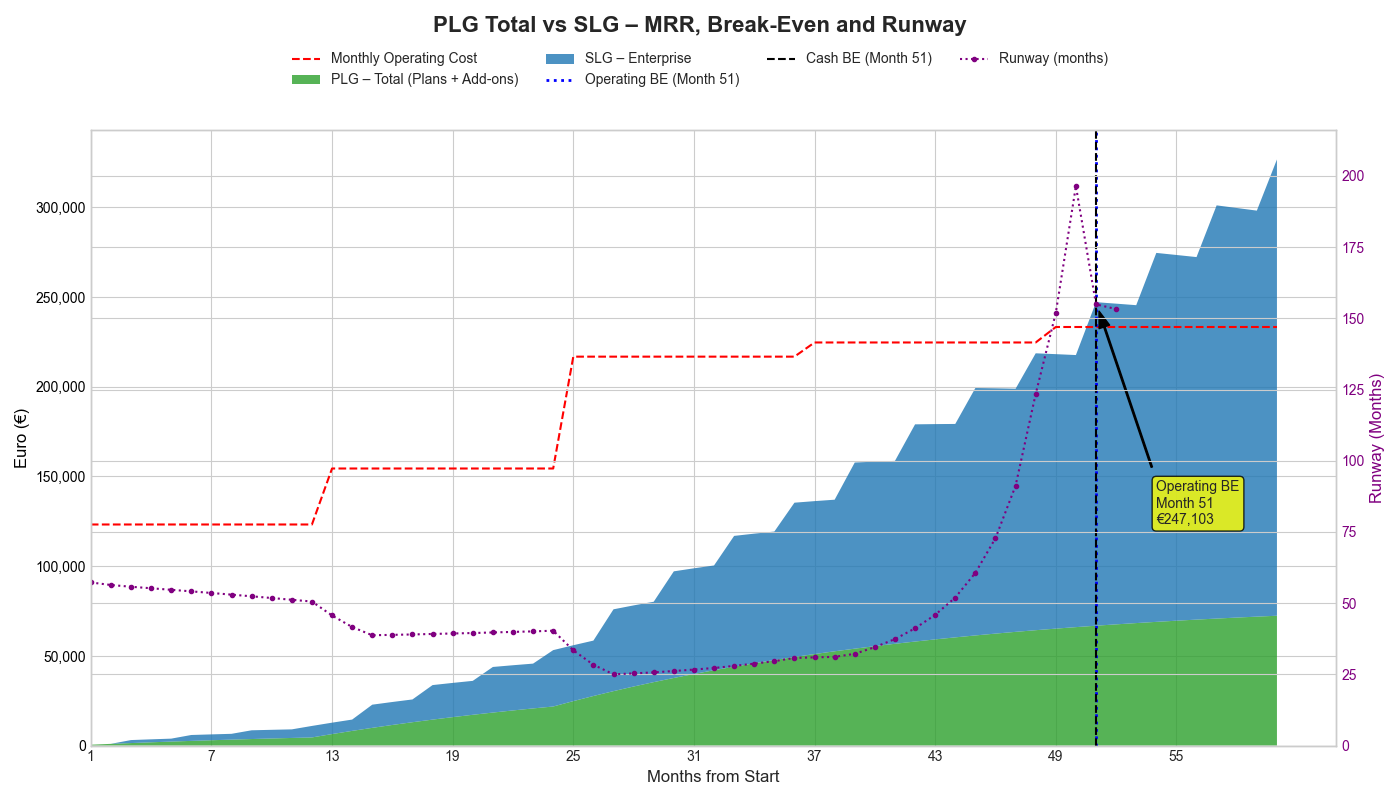
\includegraphics[width=\textwidth]{financial_projection.png}
    \caption{盈亏平衡分析:PLG 与 SLG 的 MRR、月度成本与资金跑道。}
    \label{fig:break_even_analysis}
\end{figure} 
\subsection{盈亏平衡分析:图表解读}

\paragraph{图例(速览)}
\begin{itemize}
  \item \textbf{绿色(PLG——方案 + 附加组件):} 自助式经常性收入。
  \item \textbf{蓝色(SLG——企业):} 企业经常性收入;由于年度交易被在各季度间平滑,因此以季度“阶梯”增长。
  \item \textbf{红色虚线:} 月度运营成本(包含审慎上调),按年度阶梯上升。
  \item \textbf{紫色点线:} 资金跑道(月),按现金除以3个月移动平均烧钱计算。
  \item \textbf{竖线:} 经营盈亏平衡(蓝色,第~51 月)与现金盈亏平衡(黑色,第~51 月)。
\end{itemize}

前三年图表显示的是稳健的积累。随着月度注册在流失后复利增长,且附加组件带来增量 MRR,绿色的 PLG 区域稳步上升。签订企业合同时,蓝色的 SLG 区域以可见的季度阶梯上升。成本以块状变化:每个新年增加计划产能(团队、基础设施、G\&A 并带上调),因此红线会跳升,然后在下一次阶梯前保持平坦。

这些动态与年末数据一致。年末第~1 年,成本为 \textbf{¥1{,}031{,}001}/月,对比经常性 MRR \textbf{¥91{,}610}/月(亏损 \textbf{¥938{,}429}/月,现金 \textbf{¥48{,}031{,}828},跑道 \textbf{50.6} 个月)。到第~2 年:\textbf{¥1{,}292{,}082} 对比 \textbf{¥445{,}111}(亏损 \textbf{¥843{,}924}/月),现金 \textbf{¥35{,}835{,}085},跑道 \textbf{40.3} 个月。到第~3 年:\textbf{¥1{,}813{,}666} 对比 \textbf{¥1{,}132{,}652}(亏损 \textbf{¥674{,}696}/月),现金 \textbf{¥18{,}738{,}301},跑道 \textbf{30.8} 个月。收入曲线显然在现金受控的同时逐步逼近成本:\textbf{观察到的最小跑道为 25.0 个月},且\textbf{峰值月度烧钱}为 \textbf{¥1{,}342{,}531}。

第~4 年差距显著缩小。更大的 SLG 阶梯使蓝色区域增长更快,堆叠(PLG+SLG)几乎与成本线相接。年末:成本 \textbf{¥1{,}879{,}770}/月,对比经常性 MRR \textbf{¥1{,}829{,}296}/月(总收入 \textbf{¥1{,}837{,}672}/月),几乎持平的亏损 \textbf{¥42{,}098}/月,现金 \textbf{¥18{,}738{,}301}。由于移动平均烧钱接近于零,紫色的跑道曲线开始飙升。

盈亏平衡发生在\textbf{第 51 个月}。此时\textbf{经常性 MRR 为 ¥2{,}067{,}684},成本为\textbf{¥1{,}951{,}942}(经营盈亏平衡),且\textbf{总收入 ¥2{,}076{,}520} 超过成本(现金盈亏平衡)。为达到该点,模型累计\textbf{烧钱 ¥41{,}331{,}166},且\textbf{最低现金}为 \textbf{¥18{,}698{,}236},这也代表\textbf{在盈亏平衡时的储备(融资轮的 30.9\%)}。到第~5 年末,经常性 MRR 达到 \textbf{¥2{,}733{,}267}/月($ \approx $ \textbf{¥32.80M ARR}),月度利润为 \textbf{¥791{,}292},现金为 \textbf{¥22{,}371{,}372},跑道实际上变为无限。

% ----- End of translated content from: part_15.tex -----

% ----- Start of translated content from: part_16.tex -----

\paragraph{要点}
该图清楚地表明三点:
\begin{enumerate}
\item \emph{谁推动什么} PLG 构建基础,SLG 弥合差距
\item \emph{为何成本上升} 有计划的产能阶梯与审慎上调
\item \emph{现金如何受保护} 资金跑道从不塌陷(至少 25.0 个月),并在收入超过成本后加速,完全符合所列指标。
\end{enumerate}

\begin{table}[H]
\centering
\caption{财务预测汇总(年末)}
\label{tab:financial_summary}
\resizebox{\textwidth}{!}{
\begin{tabular}{lrrrrrrr}
\toprule
\textbf{年末} & \textbf{月度成本(CNY)} & \textbf{经常性 MRR(CNY)} & \textbf{商店收入(CNY)} & \textbf{总收入(CNY)} & \textbf{月度盈亏(CNY)} & \textbf{现金余额(CNY)} & \textbf{跑道(月)} \\
\midrule
第 1 年 & 1,031,001 & 91,610 & 971 & 92,580 & -938,429 & 48,031,828 & 50.6 \\
第 2 年 & 1,292,082 & 445,111 & 3,046 & 448,157 & -843,924 & 35,835,085 & 40.3 \\
第 3 年 & 1,813,666 & 1,132,652 & 6,318 & 1,138,969 & -674,696 & 23,623,674 & 30.8 \\
第 4 年 & 1,879,770 & 1,829,296 & 8,376 & 1,837,672 & -42,098 & 18,738,301 & 123.5 \\
第 5 年 & 1,951,942 & 2,733,267 & 9,966 & 2,743,233 & 791,292 & 22,371,372 & 已盈利 \\
\bottomrule
\end{tabular}
}
\end{table}

\begin{table}[H]
\centering
\caption{关键财务指标}
\label{tab:financial_metrics}
\resizebox{\textwidth}{!}{%
\begin{tabular}{ll}
\toprule
\textbf{指标} & \textbf{数值} \\
\midrule
经营性盈亏平衡 & 第 51 个月(第 5 年):经常性 MRR CNY 2,067,684 $\geq$ 成本 CNY 1,951,942 \\
盈亏平衡 & 第 51 个月(第 5 年):总收入 CNY 2,076,520 $\geq$ 成本 CNY 1,951,942 \\
达到现金盈亏平衡前耗用资本 & CNY 41,331,166 \\
月度峰值烧钱 & CNY 1,342,363 \\
期间最低现金 & CNY 18,497,889 (30.9\% of round) \\
最短跑道(3 个月移动平均) & 25.0 个月 \\
\bottomrule
\end{tabular}
}
\end{table}

\newpage
\section{为何 CNY 59{,}829{,}055 是恰当的额度}

我们请求 \textbf{CNY 59{,}829{,}055} ($\approx\text{CNY }59.83\text{M}$),因为在我们的\emph{保守}情景下,这正是让公司在\textbf{第~51 个月实现经营与现金盈亏平衡}所需且足够的资本规模,无需强推增长,同时保留明确的安全边际。仿真结果清晰明确:\textbf{累计烧钱至现金盈亏平衡 = CNY 41{,}331{,}166},\textbf{达到平衡时的在手现金 = CNY 18{,}497{,}889}(即\textbf{30.9\%} 的轮次规模),\textbf{沿途最短跑道 = 25.0 个月}(3 个月移动平均),以及\textbf{月度峰值烧钱 = CNY 1{,}342{,}363}。我们请求的额度正是模型所示\emph{必要且充分}以在结构性预备金缓冲下达到盈亏平衡。

该计划具备韧性:成本并非“极致精简”,而是按类别(基础设施、G\&A、PLG、SLG、R\&D、管理)进行了\textbf{审慎上调},以覆盖常被低估的经常性项目(企业级支持、审计、法务、招聘、监控)。此外,模型引入了\textbf{自动护栏}:若跑道低于 12 个月,下一月\textbf{可裁量成本下调 10\%};低于 9 个月,\textbf{付费 PLG 获客降温}(乘数 0.7)。这些是写进模型的运营规则,而非口头承诺。实践中,下行由自动触发的机制所保护。

在收入侧,我们清晰区分\textbf{PLG}(套餐+附加)与\textbf{SLG}(企业)。这并非点缀:它让我们能逐月观察哪里投放更有效,并在无意识形态偏见下再平衡。在这一组合与当前定价下,\textbf{经营性盈亏平衡}在\textbf{第~51 个月}到来,彼时\textbf{经常性 MRR 为 CNY 2{,}067{,}684},对比\textbf{月度成本 CNY 1{,}951{,}942};同月实现\textbf{现金盈亏平衡},因为\textbf{总收入(CNY 2{,}076{,}520)}超过成本。到第 $\sim 5$ 年末,经常性 MRR 达到\textbf{CNY 2{,}733{,}267}($\approx$ \textbf{CNY 32.80M ARR})。就资本效率而言,\textbf{隐含烧钱倍数}(达平衡烧钱 $\div$ 达平衡时 ARR)为\textbf{约 1.66x},与保守的产品+GTM 构建相一致,且成本已被可信上调。

那么,为什么是\emph{这个}额度而不是更少?若资本更少,模型中的护栏将更频繁触发,造成运营上的走走停停(削减/冷却期),拉长时间线并提高机会成本,恰恰在连续性最重要的时候。为何不更多?因为超过此阈值后,瓶颈不在预算,而在\textbf{渠道吸纳能力}与企业交付的自然节奏;今天多拿的钱只会增加稀释,并不会相对模型改善结果。

\textbf{资金用途}严格锚定在模型中的各类目及其上调:产品/R\&D(加固、可观测性、安全)、基础设施与企业支持、SLG(客户、方案/POC)、PLG(内容/SDK/社区)、伙伴赋能、G\&A 与合规、管理。我们不会新增支出科目:我们资助的正是模型已按月度衡量的内容。 

最后,\textbf{风险画像}清晰可读。最短跑道不低于\textbf{25.0 个月},护栏在必要时限制现金流失,且在盈亏平衡时\textbf{30.9\%} 的缓冲为采购延迟、基础设施/合规支出波动或汇率波动提供了余地。同时,PLG/SLG 的分离也使得事后复盘变得直接——资本分配遵循已实现回报,而非一刀切的计划。

\textbf{简而言之:}\textbf{CNY 59{,}829{,}055} 充足覆盖保守路径下达到盈亏平衡所需,并留有足够缓冲与自动化成本纪律。这是成比例、可辩护且——最重要——\textbf{可复现}的请求:投资人可以逐月验证模型指标在控,现金按预期轨迹演进。

\subsection{战略缓冲的理由:穿越 AI 编排前沿}
盈亏平衡时 30.9\% 的资本储备(CNY 18.50M)是一种有意的战略配置,用于应对 AI 编排市场前所未有的变化速度。不同于产品市场契合路径相对可预测的传统 SaaS 赛道,AI 基础设施版图正每 3–6 个月发生根本性转变——从新的 LLM 架构到如 MCP 等新兴编排标准。该缓冲让 IntellyHub 能在不牺牲跑道的前提下快速执行战略转向:无论是适配自主体能力的突破,整合规划时尚不存在的颠覆性模型,还是根据真实市场反馈在 PLG 与 SLG 渠道间切换侧重。成功的 AI 基建公司(Weights \& Biases、Hugging Face)的历史先例表明,它们在实现可持续增长前往往需要 2–3 次重大转向——每次消耗可用资本的 15–20\%。我们的储备确保即便进行一次重大战略再定位,仍可保持 12+ 个月的运营跑道,把原本的生存威胁转化为竞争优势。这不是过剩资本;这是在唯一确定性是“激进变化”的市场中的精算化选择权保险——能比对手更快转向、而对手还在为了应急融资奔忙,正是决定市场领导或被淘汰的关键。

\newpage
\section{市场进入策略}
% 如何触达你的客户?

IntellyHub 的市场进入(GTM)策略基于“双引擎”混合模型:
\begin{enumerate}
    \item \textbf{面向 SaaS 的产品驱动增长(PLG):} 利用产品优势、免费层与 Automation Store 以自下而上、可规模化的方式吸引、激活并转化用户。
    \item \textbf{面向本地部署与企业的销售驱动增长(SLG):} 采用有针对性的顾问式销售,赢取具备复杂安全与治理需求的大客户。
\end{enumerate}
这两台引擎相互强化:PLG 的成功为销售团队带来线索与品牌声量。

% --- 战略目标 ---

% ----- End of translated content from: part_16.tex -----

% ----- Start of translated content from: part_17.tex -----

\subsection{战略目标(3年展望)}
\begin{itemize}
    \item \textbf{定位:} 成为为现代技术团队编排复杂自动化与AI工作流的领先平台。
    \item \textbf{采纳:} 围绕插件生态与自动化商店,达到活跃用户的临界规模并形成充满活力的社区。
    \item \textbf{收入:} 建立可持续的商业模式,产生可观的年度经常性收入(ARR),由SaaS订阅和企业本地部署合同共同驱动。
\end{itemize}

% --- 第1年 ---
\subsection{第1年:基础 \& 市场验证}
\textbf{主要重点:} 争取早期采用者,验证产品与市场匹配度,并拿下首批关键标杆客户(SaaS与本地部署均包括)。在此阶段,许多活动是人工且“不可规模化。”

\newpage
\begin{table}[H]
\centering
\resizebox{\textwidth}{!}{
\begin{tabularx}{\textwidth}{L L L} 
\toprule
\textbf{关键渠道} & \textbf{具体行动} & \textbf{成功KPI} \\

\midrule
\textbf{产品驱动增长(PLG)} & 
\textbf{细分市场发布:} 在 Product Hunt、Hacker News 以及相关技术子版块(如 r/devops、r/kubernetes)等平台展示 IntellyHub。\newline\newline
\textbf{自动化商店:} 充实商店,提供20-30个高质量官方模板,解决真实痛点问题。
&
\textbf{激活率:} >25\%(用户在7天内运行其首个自动化)。\newline\newline
\textbf{1个月留存率:} >15\%(4周后回访的用户)。
\\
\addlinespace

\textbf{技术内容营销} & 
\textbf{博客 \& 教程:} 每月发布2-4篇深度技术文章,展示如何用 IntellyHub 解决特定问题。\newline\newline
\textbf{视频内容:} 制作简明的视频教程。
&
\textbf{优质流量:} 来自自然与推荐渠道的网站访问量。\newline\newline
\textbf{访客转注册率:} >2\%.
\\
\addlinespace

\textbf{社区建设} &
\textbf{Discord/Slack 频道:} 为早期用户建立一个中心枢纽。\newline\newline
\textbf{创始人主导支持:} 亲自回答每一个问题和反馈请求,建立牢固的关系。
&
\textbf{社区参与度:} 每周活跃成员数、点对点支持互动数。\newline\newline
\textbf{定性反馈:} 每月至少开展5次深入的用户访谈。
\\
\addlinespace

\textbf{创始人主导销售(本地部署)} &
\textbf{利用人脉:} 创始人亲自与其人脉中的目标公司推进前3-5个销售流程。\newline\newline
\textbf{概念验证(POC):} 专注于少数高价值POC的成功。
&
\textbf{已启动的POC:} 全年3-5个。\newline\newline
\textbf{签署的本地部署合同:} 1-2个关键标杆客户。
\\
\bottomrule
\end{tabularx}
}
\end{table}


% --- 第2年 ---
\newpage
\subsection{第2年:扩张 \& 构建可复制的增长引擎}
\textbf{主要重点:} 将初始价值转化为可扩展、可重复的流程。优化第1年行之有效的方法,并为商业化团队打下基础。

\begin{table}[H]
\small
\centering
\resizebox{\textwidth}{!}{
\begin{tabularx}{\textwidth}{L L L}
\toprule
\textbf{关键渠道} & \textbf{具体行动} & \textbf{成功KPI} \\
\midrule
\textbf{PLG 优化} &

\textbf{漏斗分析:} 使用分析工具识别并消除从注册到付费转化过程中的摩擦点。
\textbf{引导式上手:} 在应用内实施引导式入门体验,带领新用户达到他们的 "Aha!" 时刻。
&

\textbf{免费转付费转化率:} >3\%.

% ----- End of translated content from: part_17.tex -----

% ----- Start of translated content from: part_18.tex -----

\textbf{MRR 增长率:} 持续的环比增长。
\\
\addlinespace
\textbf{生态合作伙伴关系} &

\textbf{战略集成:} 为 2-3 个拥有相似用户群的互补技术平台积极开发插件。
\textbf{联合营销:} 与合作伙伴发起联合营销活动(网络研讨会、博客文章)。
&

\textbf{合作伙伴来源线索。}
\textbf{合作伙伴插件下载量。}
\\
\addlinespace
\textbf{初始销售团队} &

\textbf{首批招聘:} 再招聘客户经理以处理入站线索,并开始有针对性的外呼开发。
\textbf{销售手册:} 根据创始人主导销售阶段的经验,规范化销售流程。
&

\textbf{每月合格演示次数。}
\textbf{平均销售周期长度(本地部署)。}
\\
\bottomrule
\end{tabularx}
}
\end{table}

\newpage
% --- 第 3 年 ---
\subsection{第 3 年:扩张 \& 细分市场领导力}
\textbf{主要关注点:} 加速增长,占领技术团队细分领域,并将 IntellyHub 打造成 AI 编排市场的思想领袖。

\begin{table}[H]
\centering
\resizebox{\textwidth}{!}{
\begin{tabularx}{\textwidth}{L L L}
\toprule
\textbf{关键渠道} & \textbf{具体行动} & \textbf{成功 KPI} \\
\midrule
\textbf{销售可扩展性} &

\textbf{团队扩张:} 扩充销售团队,以覆盖不同地域或行业垂直领域。
\textbf{间接渠道:} 开始探索与系统集成商和经销商的合作关系。
&

\textbf{年度经常性收入(ARR)增长。}
\textbf{获客成本(CAC)与 LTV/CAC 比率。}
\\
\addlinespace
\textbf{品牌营销} &

\textbf{思想领导力:} 基于平台汇总数据发布行业报告。
\textbf{赞助:} 赞助 DevOps 与 AI 领域的关键会议和播客。
&

\textbf{行业媒体提及次数。}
\textbf{直接流量 \& 品牌流量的增长。}
\\
\addlinespace
\textbf{网络效应} &

\textbf{开放商店:} 将自动化商店和插件市场向外部贡献开放,并为合作伙伴提供认证。
\textbf{开发者计划:} 启动正式的开发者关系(DevRel)项目。
&

\textbf{社区创建的插件/模板数量。}
\textbf{净收入留存率(NRR):} >110\%。
\\
\bottomrule
\end{tabularx}
}
\end{table}

\clearpage
\section{运营计划}
% 公司将如何在日常层面运作。
\subsection{引言}
本文档概述了执行 IntellyHub 的产品开发与市场进入战略的运营计划。该计划与产品开发路线图的各阶段保持一致,并描述了公司各职能领域的关键活动。

% --- 第 1 阶段 ---

% ----- End of translated content from: part_18.tex -----

% ----- Start of translated content from: part_19.tex -----

\subsection{阶段1: 基础与验证 (第1-2季度)}
\textbf{战略目标:} 将原型转化为稳定且安全的MVP,获取首批早期采用者,并通过有针对性的合作伙伴计划\textbf{验证核心产品与定价模型假设。}

\subsubsection{产品开发 \& 工程}
\begin{itemize}[leftmargin=*]
    \item \textbf{Q1:}
    \begin{itemize}
        \item \textbf{稳定性:} 完成测试套件(单元、集成),以确保核心引擎的可靠性。
        \item \textbf{插件:} 完成并文档化内部系统,以支持标准化的插件开发。
        \item \textbf{UI/UX:} 打磨混合式IDE界面,解决任何同步问题并提升用户体验。
        \item \textbf{本地部署:} 为企业客户开发并测试平台的本地部署版本。
    \end{itemize}
    \item \textbf{Q2:}
    \begin{itemize}
        \item \textbf{认证:} 实现健壮的用户管理与认证系统。
        \item \textbf{引导上手:} 为新用户开发引导式入门向导。
        \item \textbf{商店 (v1):} 为自动化商店的第一版 (只读) 创建API与UI。
    \end{itemize}
\end{itemize}

\subsubsection{市场进入 (市场 \& 销售)}
\begin{itemize}[leftmargin=*]
    \item \textbf{Q1-Q2:}
    \begin{itemize}
        \item \textbf{垂直策略:} 在\textit{初始垂直细分领域}内定义详尽的理想客户画像 (ICP)(例如: 生物技术/科学研究,基于 Esplorado 的用户案例)。
        \item \textbf{(新) 设计合作伙伴计划:} 面向目标垂直领域遴选的3-5家公司推出专属计划。提供早期访问与直接支持,以换取持续反馈及潜在的初步合同。
    \end{itemize}
    \item \textbf{Q3-Q4:}
    \begin{itemize}
        \item \textbf{细分市场发布:} 在 Product Hunt、Hacker News 及相关渠道进行发布,沟通聚焦所选垂直领域。
        \item \textbf{反馈收集:} 从免费层用户以及优先的设计合作伙伴处收集结构化反馈。
    \end{itemize}
\end{itemize}

\subsubsection{社区 \& 生态系统管理}
\begin{itemize}[leftmargin=*]
    \item \textbf{Q1-Q2:}
    \begin{itemize}
        \item \textbf{定向插件开发:} 开发并文档化首批 "官方" 插件,\textit{优先考虑与目标垂直领域最相关的插件}。
    \end{itemize}
    \item \textbf{Q3-Q4:}
    \begin{itemize}
        \item \textbf{社区创建:} 启动官方 Discord/Slack 服务器。
        \item \textbf{互动参与:} 创始人和开发团队将积极参与,解答问题并营造友好的社区氛围。
    \end{itemize}
\end{itemize}

\subsubsection{通用事务 \& 公司运营}
\begin{itemize}[leftmargin=*]
    \item \textbf{Q1-Q2:}
    \begin{itemize}
        \item \textbf{法律与行政设置:} 完成公司架构设定,开立银行账户。
        \item \textbf{(新) 合作伙伴合同:} 为 "设计合作伙伴计划" 准备相关协议。
    \end{itemize}
    \item \textbf{Q3-Q4:}
    \begin{itemize}
        \item \textbf{服务条款制定:} 为免费层发布撰写并发布服务条款与隐私政策。
    \end{itemize}
\end{itemize}

\clearpage

% --- PHASE 2 ---
\subsection{阶段2: 扩张与增长 (第3-4季度)}
\textbf{战略目标:} 基于阶段1验证的数据,扩大用户获取规模,拓展生态系统,并实现为商业化所需的企业级功能。

\subsubsection{产品开发 \& 工程}
\begin{itemize}[leftmargin=*]
    \item \textbf{Q5-Q6:}
    \begin{itemize}
        \item \textbf{安全:} 实施用于凭据的机密管理系统。
        \item \textbf{版本控制:} 为自动化添加历史与回滚功能。
    \end{itemize}
    \item \textbf{Q7-Q8:}
    \begin{itemize}
        \item \textbf{可观测性:} 开发用于流程性能度量的数据平台第一版。
        \item \textbf{改进仪表板:} 创建用于可视化流程的用户界面。
        \item \textbf{主动式AI:} 基于流程性能数据实现基础的 "自愈" 功能。
    \end{itemize}
\end{itemize}

% ----- End of translated content from: part_19.tex -----

% ----- Start of translated content from: part_20.tex -----

\subsubsection{进入市场(市场营销 \& 销售)}
\begin{itemize}[leftmargin=*]
    \item \textbf{Q5-Q6:}
    \begin{itemize}
        \item \textbf{垂直内容营销:} 扩大针对所选垂直领域的内容产出(基于设计合作伙伴的案例研究、文章)。
        \item \textbf{招聘:} 启动首位开发者布道师的招聘流程。
    \end{itemize}
    \item \textbf{Q7-Q8:}
    \begin{itemize}
        \item \textbf{付费方案发布:} 敲定定价(与设计合作伙伴验证)并正式推出专业版与企业版方案。
        \item \textbf{销售作战手册(v1):} 开始记录面向企业客户的销售流程。
    \end{itemize}
\end{itemize}

\clearpage

% --- 阶段 3 ---
\subsection{第3阶段:领导力与创新(第5-6季度)}
\textbf{战略目标:} 确立市场领导地位,通过社区创造网络效应,并**利用数据构建不可逾越的竞争优势。**

\subsubsection{产品开发 \& 工程}
\begin{itemize}[leftmargin=*]
    \item \textbf{Q9-Q10:}
    \begin{itemize}
        \item \textbf{商店开放:} 开放商店,允许社区提交内容。
        \item \textbf{内容审核:} 构建内部工具,用于审核和验证外部贡献。
    \end{itemize}
    \item \textbf{Q11-Q12:}
    \begin{itemize}
        \item \textbf{(修订版)数据平台 \& 可观测性:} 开发用于收集和汇总流程性能指标的系统,其战略目标是\textbf{构建 "数据护城河"}。
        \item \textbf{分析仪表盘:} 创建用于可视化分析的用户界面。
        \item \textbf{主动式 AI:} 改进 "自愈" 和主动优化功能,\textbf{基于聚合的平台数据进行训练}。
    \end{itemize}
\end{itemize}

\subsubsection{进入市场(市场营销 \& 销售)}
\begin{itemize}[leftmargin=*]
    \item \textbf{Q9-Q10:}
    \begin{itemize}
        \item \textbf{销售团队扩张:} 招聘更多客户经理以覆盖特定市场或垂直领域。
        \item \textbf{思想领导力:} 开始发布基于平台使用数据的报告与分析。
    \end{itemize}
    \item \textbf{Q11-Q12:}
    \begin{itemize}
        \item \textbf{品牌营销:} 加大在品牌认知活动(赞助、活动)上的投入。
    \end{itemize}
\end{itemize}

\newpage
\section{风险分析}
\subsection{市场风险}
\textit{与市场、竞争和客户采用相关的风险。}

\begin{table}[H]
\centering
\begin{tabularx}{\textwidth}{@{}lL@{}}
\toprule
\textbf{风险} & \textbf{描述} \\
\midrule
\textbf{来自 "现状" 的竞争} & 我们最大的竞争对手并非另一家平台,而是开发者使用自定义 Python 脚本的惰性。他们的熟悉度以及被认为为零的初始成本,使之成为一大障碍。 \\
\addlinespace
\textbf{企业采用周期缓慢} & 本地部署和企业销售模式对于高价值合同至关重要,但其特点是冗长的销售周期(6-12 个月以上)以及复杂的概念验证(POC)阶段。首批关键企业交易的成交延迟可能会显著影响收入预测。 \\
\addlinespace
\textbf{AI 技术转变} & 我们的 AI 目前定位为“副驾驶”。若竞争对手迅速实现向“足够好”的真正自主 AI 代理的技术飞跃,可能会使我们更受控、结构化的方法显得不那么创新。 \\
\bottomrule
\end{tabularx}
\end{table}

\newpage
\subsection{运营风险}
\textit{与技术、人员和执行相关的风险。}

\begin{table}[H]
\centering
\begin{tabularx}{\textwidth}{@{}lL@{}}
\toprule
\textbf{风险} & \textbf{描述} \\
\midrule
\textbf{团队执行 \& 关键人员风险} & 该计划依赖于招聘少量高度专业化的人才。项目的成功在很大程度上取决于这一核心团队在产品、基础设施和销售方面的执行能力。关键成员的离职可能导致重大延误。 \\

% ----- End of translated content from: part_20.tex -----

% ----- Start of translated content from: part_21.tex -----

\addlinespace
\textbf{技术复杂性} & 技术栈(Kubernetes、多步AI流水线、混合式IDE)功能极其强大,但维护与演进同样复杂。在这样的复杂系统中,缺陷、安全漏洞或性能瓶颈往往难以排查且修复成本高昂。 \\
\addlinespace
\textbf{混合技术风险(IDE/YAML 同步)} & 在复杂的可视化IDE与文本化YAML表示之间维持完美、实时、双向的同步在技术上要求极高。这可能成为细微且难以调试的缺陷来源,影响用户信任。 \\
\addlinespace
\textbf{生态质量控制} & 自动化商店与插件市场的价值是一把双刃剑。低质量、不安全或维护不善的社区贡献可能损害用户信任与平台声誉。 \\
\bottomrule
\end{tabularx}
\end{table}

\newpage
\subsection{财务风险}
\textit{与现金流、融资及财务可持续性相关的风险。}

\begin{table}[H]
\centering
\begin{tabularx}{\textwidth}{@{}lL@{}}
\toprule
\textbf{风险} & \textbf{描述} \\
\midrule
\textbf{初期烧钱率高} & 激进的招聘计划在产生可观收入之前就带来高额月度运营成本。这迫使团队在巨大压力下快速实现产品市场匹配并尽快产生收入。 \\
\addlinespace
\textbf{融资依赖} & 商业模式并非面向短期盈利设计。未能达成投资人期望的增长KPI将构成生存威胁。 \\
\addlinespace
\textbf{定价模型验证} & 所提出的价值度量(执行次数、活跃自动化)合乎逻辑但尚未验证。不当的定价模型可能导致客户阻力(过贵时)或错失可观收入(过便宜时)。 \\
\bottomrule
\end{tabularx}
\end{table}

\newpage
\subsection{缓解策略}
\textit{用于应对并降低已识别风险的具体行动。}

\begin{table}[H]
\centering
\begin{tabularx}{\textwidth}{@{}lL@{}}
\toprule
\textbf{风险类别} & \textbf{缓解策略} \\
\midrule
\textbf{市场风险} & 
\textbf{定位与教育:} 市场推广应聚焦于消除管理\textit{大量}脚本的长期混乱,而非替代单个脚本。利用诸如“Esplorado”等案例研究提供无可辩驳的价值证明。 \newline\newline
\textbf{混合GTM:} 并行推进PLG(SaaS)与SLG(本地部署)路径。利用PLG端更快的反馈循环,为较慢的企业销售周期打磨产品与信息传达。 \newline\newline
\textbf{战略性AI路线图:} 将当前AI定位为面向生产环境的务实、安全、可靠之选。将路线图表述为迈向更高自主能力的演进,并以当下稳固的基础为依托。 \\
\addlinespace
\textbf{运营风险} & 
\textbf{文档与交叉培训:} 从第一天起就大力投入内部文档建设。推行知识共享与结对编程文化,以降低对单一个体的依赖。 \newline\newline
\textbf{投入可观测性与测试:} 投入资源建设健壮的自动化测试套件,并尽早集成APM(应用性能监控)工具,以前瞻性识别并解决问题。测试套件应重点覆盖IDE/YAML同步逻辑。 \newline\newline
\textbf{策展式生态:} 初期商店仅收录“官方”和“认证合作伙伴”的插件。为后续所有社区提交实施明确且严格的审核流程,包括自动化安全扫描与质量检查。 \\
\addlinespace
\textbf{财务风险} & 
\textbf{基于里程碑的支出:} 将主要开支增长(尤其是市场与销售招聘)与预先定义的具体里程碑挂钩(例如拿下前10位付费客户、达到某一留存率)。 \newline\newline
\textbf{持续的投资者关系:} 与现有及潜在投资者保持透明、常态化的沟通渠道,分享KPI进展,以建立信心并顺利推进下一轮融资。 \newline\newline
\textbf{定价迭代:} 以简单、灵活的定价模型起步。直接与早期客户互动,理解其获得的价值,并根据其反馈与使用数据随时准备迭代定价结构。 \\
\bottomrule
\end{tabularx}
\end{table}

% \newpage
% \subsection{产品截图}
% 产品的截图、模型或示意图。

\newpage
% 在此添加文档中引用的来源、研究或文章。
\begin{thebibliography}{99}
    \bibitem{AIMarket}
    Market.us, \textit{自动化机器学习市场报告}, 可访问:\url{https://market.us/report/automated-machine-learning-market/}, 2025年March~2025.
    
    \bibitem{MLOpsMarket}
    MarketReserchFuture.com, \textit{MLOps市场研究报告:按组件(服务、平台)、按部署方式(本地、云)、按组织规模(大型企业、中小企业)、按行业(BFSI〔银行、金融服务与保险〕、零售与电商、政府与国防、医疗与生命科学、制造业及其他)以及按地区(北美、欧洲、亚太及世界其他地区)——市场预测至2034年。}, 可访问:\url{https://www.marketresearchfuture.com/reports/mlops-market-18849}, 2025年Agoust~2025.
    
    \bibitem{AIOrch}
    Market.us, \textit{AI编排平台市场报告(2024--2034年预测)}, 2025年February~2025.  
    可访问:\url{https://market.us/report/ai-orchestration-platform-market/}.

    \bibitem{GartnerAgentic}
    Reuters(援引Gartner), \textit{到2027年,超过40\%的代理式AI项目将被废弃……到2028年,33\%的企业软件将包含代理式AI,且15\%的决策将实现自主化,} 2025年June~25,~2025.  
    可访问:\url{https://www.reuters.com/business/over-40-agentic-ai-projects-will-be-scrapped-by-2027-gartner-says-2025-06-25/}.

    \bibitem{MLOpsMM}
    MarketsandMarkets Research, \textit{预计到2027年MLOps市场规模将突破US\$5.9 Billion,复合年增长率达41.0\%}, 2023年April~21,~2023.

% ----- End of translated content from: part_21.tex -----

% ----- Start of translated content from: part_22.tex -----

可在以下网址获取:\url{https://www.globenewswire.com/news-release/2023/04/21/2652028/0/en/MLOps-Market-Size-is-Anticipated-to-Cross-US-5-9-billion-by-2027-growing-at-a-CAGR-of-41-0-Report-by-MarketsandMarkets.html}.

    \bibitem{ModelOpsGV}
    Grand View Research,\textit{ModelOps 市场报告},2025 年版。  
    可在以下网址获取:\url{https://www.grandviewresearch.com/industry-analysis/modelops-market-report}.

    \bibitem{AIMLMarket}
    Market.us,\textit{自动化机器学习市场报告(2024--2034 年预测)},三月~2025年。  
    可在以下网址获取:\url{https://market.us/report/automated-machine-learning-market/}.

    \bibitem{MLOpsMRF}
    MarketResearchFuture,\textit{MLOps 市场研究报告(2024--2034 年预测)},八月~2025年。  
    可在以下网址获取:\url{https://www.marketresearchfuture.com/reports/mlops-market-18849}.

    \bibitem{deloitte2020}
    Deloitte,\textit{智能边缘助力的自动化:超级赋能企业的新前沿},2020 年。可在以下网址获取:\url{https://www2.deloitte.com/us/en/insights/topics/talent/intelligent-automation-2020-survey-results.html}

    \bibitem{grandviewRPA}
    Grand View Research,\textit{机器人流程自动化(RPA)市场规模、份额 \& 趋势分析报告},2024 年。可在以下网址获取:\url{https://www.grandviewresearch.com/industry-analysis/robotic-process-automation-rpa-market}

    \bibitem{mckinseyAI2023}
    McKinsey \& Company,\textit{2023 年 AI 现状:生成式 AI 的爆发之年},2023 年 8 月 1 日。可在以下网址获取:\url{https://www.mckinsey.com/capabilities/quantumblack/our-insights/the-state-of-ai-in-2023-generative-ais-breakout-year}


    \bibitem{langchainGitHub}
    LangChain GitHub 代码库。可在以下网址获取:\url{https://github.com/langchain-ai/langchain}

    \bibitem{gartnerAIBarriers}
    Gartner,\textit{AI 采用的两大障碍},2021 年 11 月 2 日。可在以下网址获取:\url{https://www.gartner.com/en/articles/2-barriers-to-ai-adoption}

    \bibitem{euAIAct}
    European Commission,\textit{人工智能监管框架提案}。可在以下网址获取:\url{https://digital-strategy.ec.europa.eu/en/policies/regulatory-framework-ai}
    
    \bibitem{AIOrch}
    Market.us,\textit{AI 编排平台市场报告(2024--2034 年预测)},二月~2025年。可在以下网址获取:\url{https://market.us/report/ai-orchestration-platform-market/}.

    \bibitem{zapierApps}
    Zapier,\textit{探索 6,000+ 个应用}。可在以下网址获取:\url{https://zapier.com/apps}

    \bibitem{g2ZapierReviews}
    G2,\textit{Zapier 评价}。可在以下网址获取:\url{https://www.g2.com/products/zapier/reviews}

    \bibitem{zapierPricing}
    Zapier,\textit{Zapier 定价方案}。可在以下网址获取:\url{https://zapier.com/pricing}


    \bibitem{zapierOpenAI}
    Zapier,\textit{OpenAI 集成}。可在以下网址获取:\url{https://zapier.com/apps/openai/integrations}

    \bibitem{g2MakeVsZapier}
    G2,\textit{对比 Make 与 Zapier}。可在以下网址获取:\url{https://www.g2.com/compare/make-vs-zapier}


    \bibitem{autogenGitHub}
    Microsoft,\textit{AutoGen GitHub 代码库}。可在以下网址获取:\url{https://github.com/microsoft/autogen}

    \bibitem{crewaiGitHub}
    Joao Moura,\textit{CrewAI GitHub 代码库}。可在以下网址获取:\url{https://github.com/joaomdmoura/crewAI}

    \bibitem{langchainValuation}
    TechCrunch,\textit{AI 基础设施初创公司 LangChain 据报道以 $1.1B 估值融资 $100M},2025 年 7 月 9 日。可在以下网址获取:\url{https://siliconangle.com/2025/07/09/ai-infrastructure-startup-langchain-reportedly-raises-100m-1-1b-valuation/#:~:text=Artificial%20intelligence%20infrastructure%2C%20developer%20tools,on%20a%20%241.1%20billion%20valuation.}

    \bibitem{langchainIntegrations}
    LangChain Documentation,\textit{LangChain 集成}。可在以下网址获取:\url{https://python.langchain.com/docs/integrations/providers/}

    \bibitem{langchainCritique}
    Medium,\textit{LangChain 的挑战 \& 批评},2025 年 3 月 3 日。可在以下网址获取:\url{https://shashankguda.medium.com/challenges-criticisms-of-langchain-b26afcef94e7}

    \bibitem{mrfRPA}
    Market Research Future,\textit{机器人流程自动化(RPA)市场研究报告信息:按流程(决策支持、自动化解决方案和管理解决方案)、按运营(基于规则和基于知识)、按行业(制造 \& 物流,以及 IT \& 电信)以及按地区(北美、欧洲、亚太和世界其他地区)–行业规模、份额及至 2032 年的预测}。可在以下网址获取:\url{https://www.marketresearchfuture.com/reports/robotic-process-automation-market-2209}

    \bibitem{uipathGartner}
    UiPath,\textit{RPA 的 Gartner 魔力象限},2025 年。可在以下网址获取:
    \url{https://www.uipath.com/resources/automation-analyst-reports/gartner-magic-quadrant-robotic-process-automation}

    \bibitem{awsSagemaker}
    Amazon AWS SageMaker,\textit{Amazon SageMaker},可在以下网址获取:\url{https://aws.amazon.com/sagemaker/}

    \bibitem{forresterRPAvsAI}
    Craig Le Clair,\textit{RPA 平台会继续保持相关性吗?AI 代理或许给出答案},Forrester,2024 年 4 月 25 日。可在以下网址获取:\url{https://www.forrester.com/blogs/will-rpa-platforms-remain-relevant-ai-agents-may-hold-the-answer/}

% ----- End of translated content from: part_22.tex -----

% ----- Start of translated content from: part_23.tex -----

\end{thebibliography}


\end{document}

% ----- End of translated content from: part_23.tex -----

